\documentclass{article}
\usepackage[10pt]{extsizes}
\usepackage[utf8]{inputenc}
\usepackage[russian]{babel}
\usepackage{amsmath}
\usepackage{amssymb}
\usepackage{graphicx}
\usepackage{listings}
\usepackage{hyperref}
\usepackage{ragged2e}
\usepackage{tabularx}
\usepackage{xlop}
\DeclareMathOperator{\gcd}{gcd}
\usepackage[left=30mm, top=20mm, right=15mm, bottom=20mm, nohead, nofoot]{geometry}
\begin{document}

\section*{Типовик Сухов Н., 368876}
\section*{1.1}
Напишите программу которая на основе веденной таблицы выводит полином жегалкина. Формат ввода: вводится n количество переменных и $2^n$ строк по $n+1$ нулей или единиц (таблица истинности).
Пример ввода:
\begin{lstlisting}[language=bash]
2
0 0 0
1 0 1
0 1 1
1 1 1
\end{lstlisting}
Пример вывода:
\begin{lstlisting}[language=bash]
a+b+ab
\end{lstlisting}
\textbf{Решение}: \url{https://github.com/n-sukhov/ITMO-courses/blob/main/Discrete%20Mathematics/1.1.cpp}

\section*{1.2}
Постройте полиномы жегалкина 15 различным функциям от четырех переменных.
\begin{itemize}
    \item $P_{1}=a\oplus b \oplus c\oplus d$
    \item $P_{2}=abcd$
    \item $P_{3}=ab\oplus cd$
    \item $P_{4}=abc\oplus d$
    \item $P_{5}=1\oplus a$
    \item $P_{6}=1\oplus b$
    \item $P_{7}=1\oplus c$
    \item $P_{8}=1\oplus d$
    \item $P_{9}=1\oplus abcd$
    \item $P_{10}=ab\oplus bc\oplus acd$
    \item $P_{11}=a\oplus ab\oplus cd$
    \item $P_{12}=ad\oplus bcd$
    \item $P_{13}=1\oplus abd$
    \item $P_{14}=ad\oplus acd\oplus c$
    \item $P_{15}=a\oplus bcd$
\end{itemize}
\section*{2.1}
Для введенного графа определить отношение рефлексивное, транзитивное
и симметричное. Формат ввода: вводится $n$ число ребер и $m$ число вершин. На следующих $n$ строках вводится пары чисел. Пара чисел означает куда и откуда идет ребро.
Пример ввода:
\begin{lstlisting}[language=bash]
33
12
23
31
\end{lstlisting}
Пример вывода:\\
\\
\texttt{Рефлексивное}\\
\texttt{Транзитивное}\\
\texttt{Антисимметричное}
\\
\\
\textbf{Решение}: \url{https://github.com/n-sukhov/ITMO-courses/blob/main/Discrete%20Mathematics/2.1.cpp}

\section*{2.2}
Определите для 15 различных графов из 10 вершин и 20 ребер являются
ли они рефлексивными, тразитивными и симметричными.

\begin{figure}[h]
    \centering
    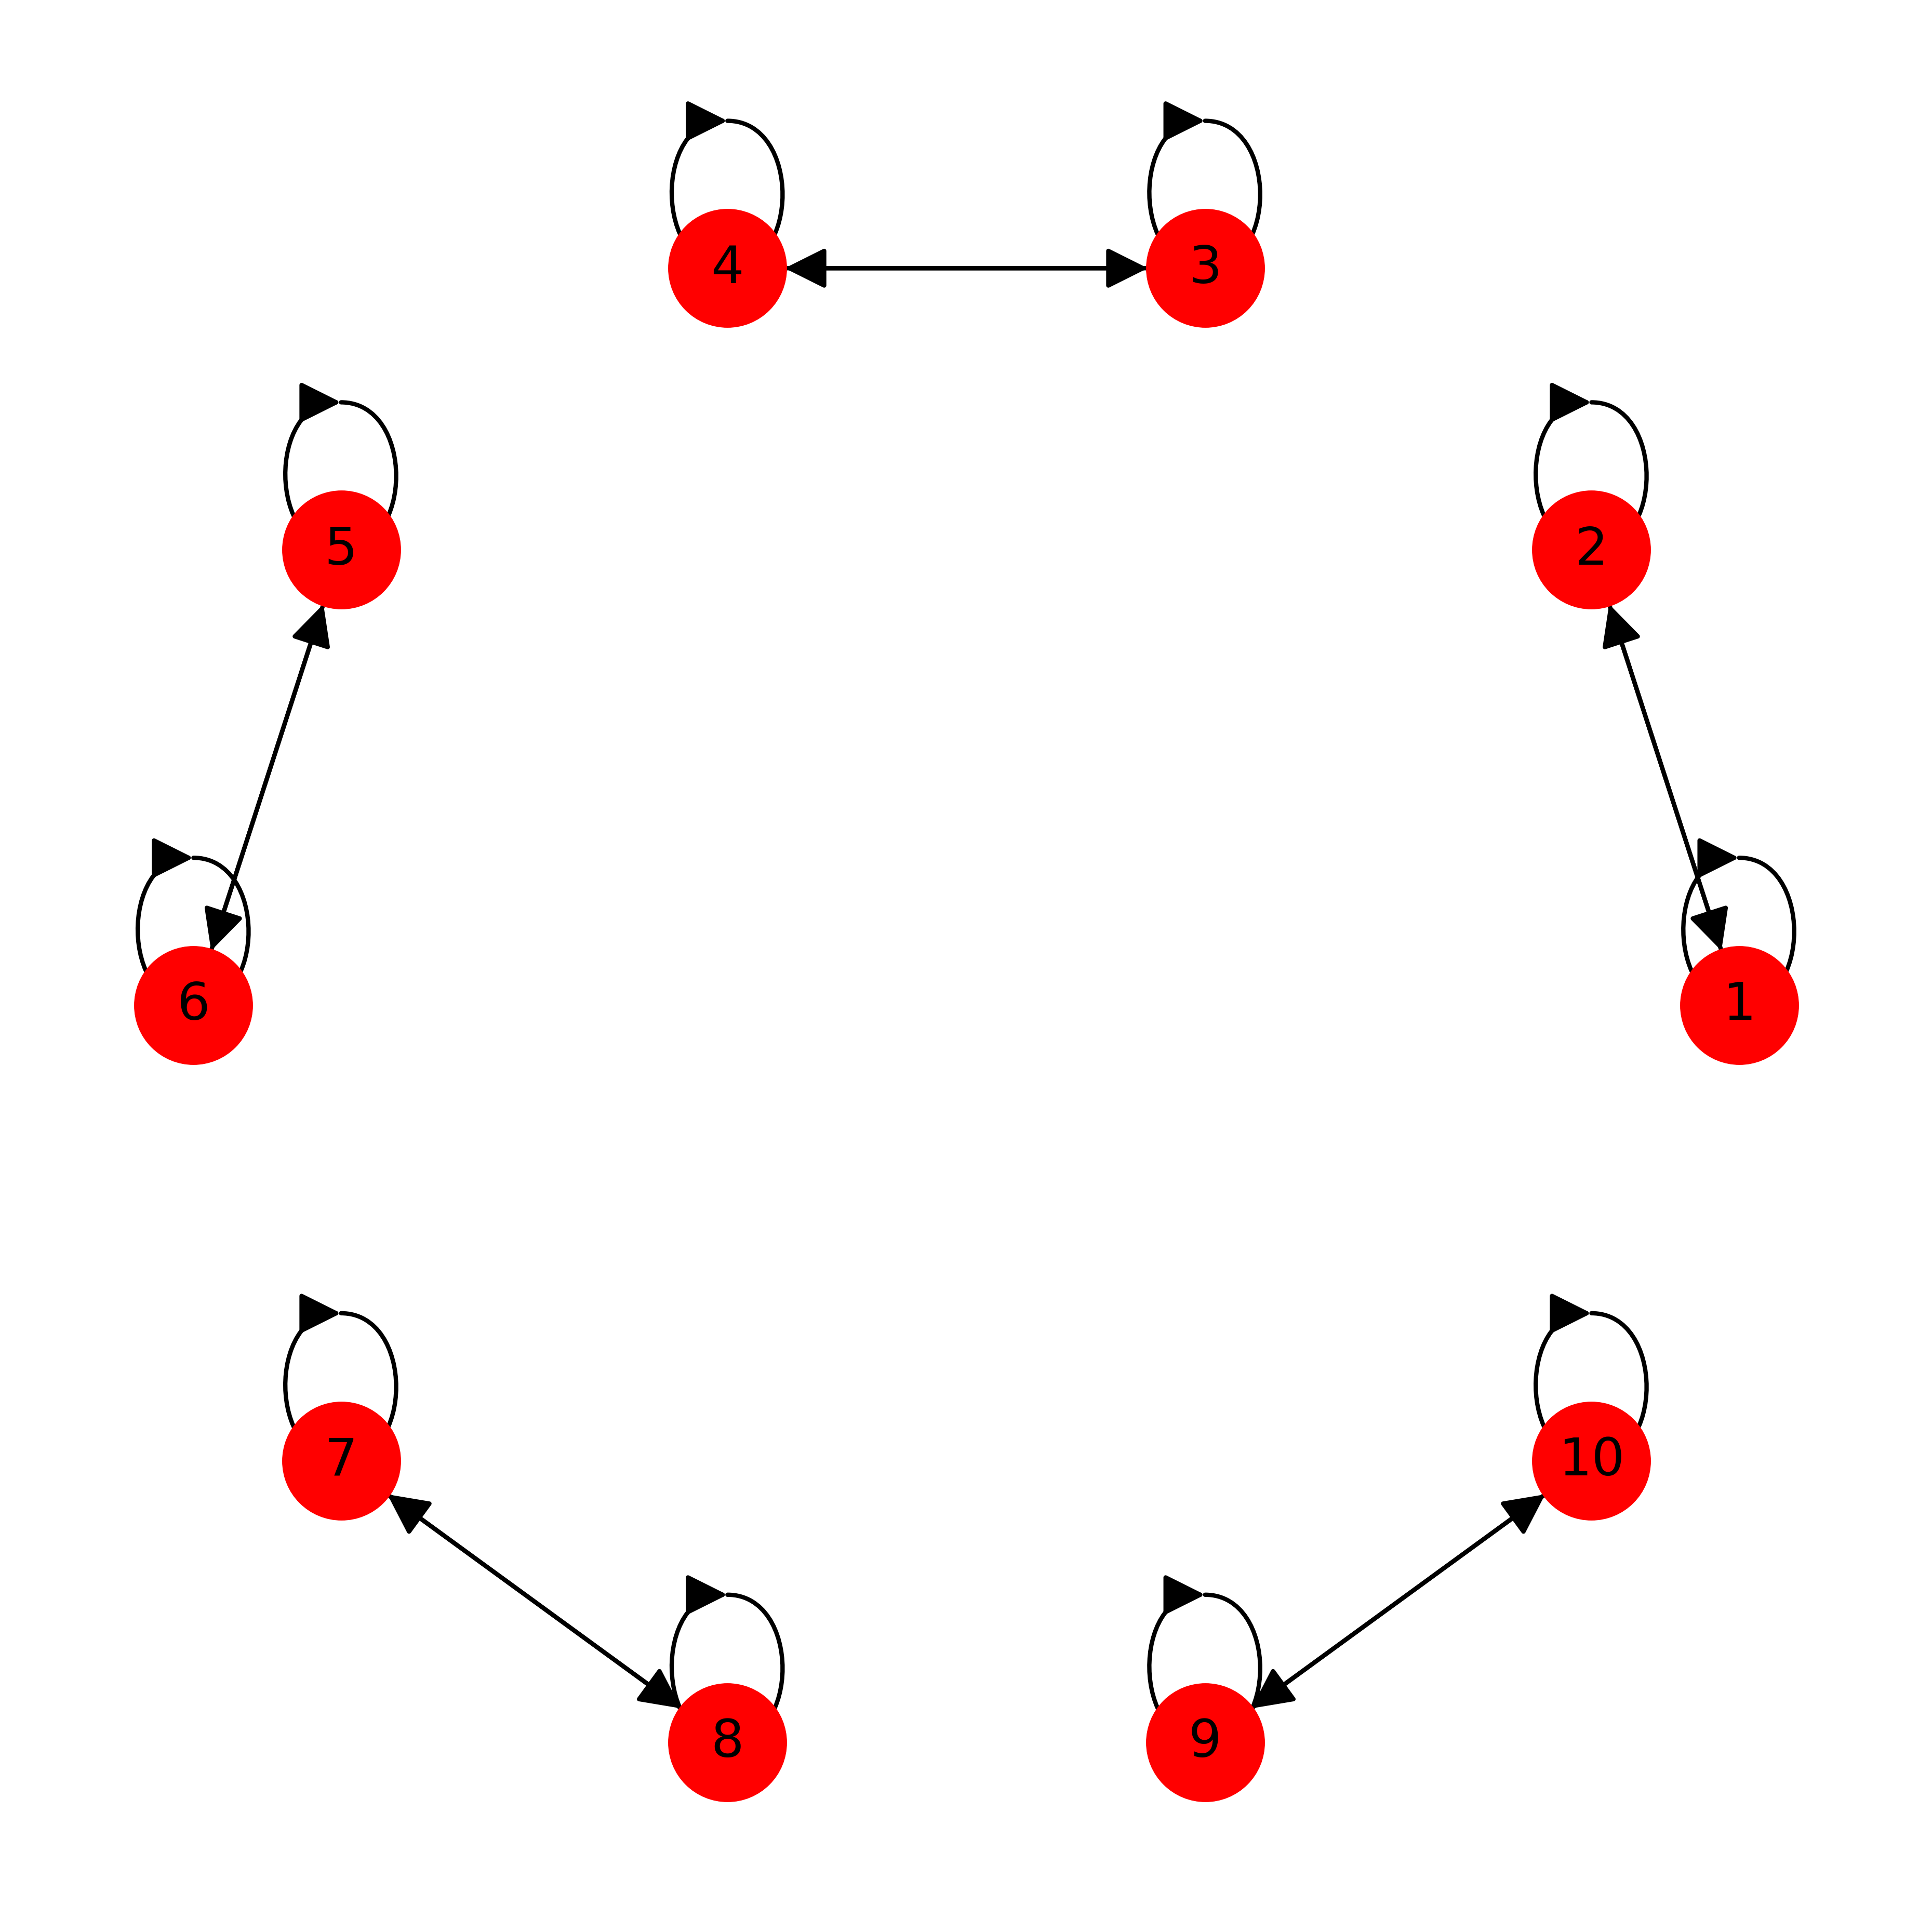
\includegraphics[width=0.4\linewidth]{img/1.png}
    \caption{Рефлексивный, Транзитивный, Симметричный}
\end{figure}

\begin{figure}[h]
    \centering
    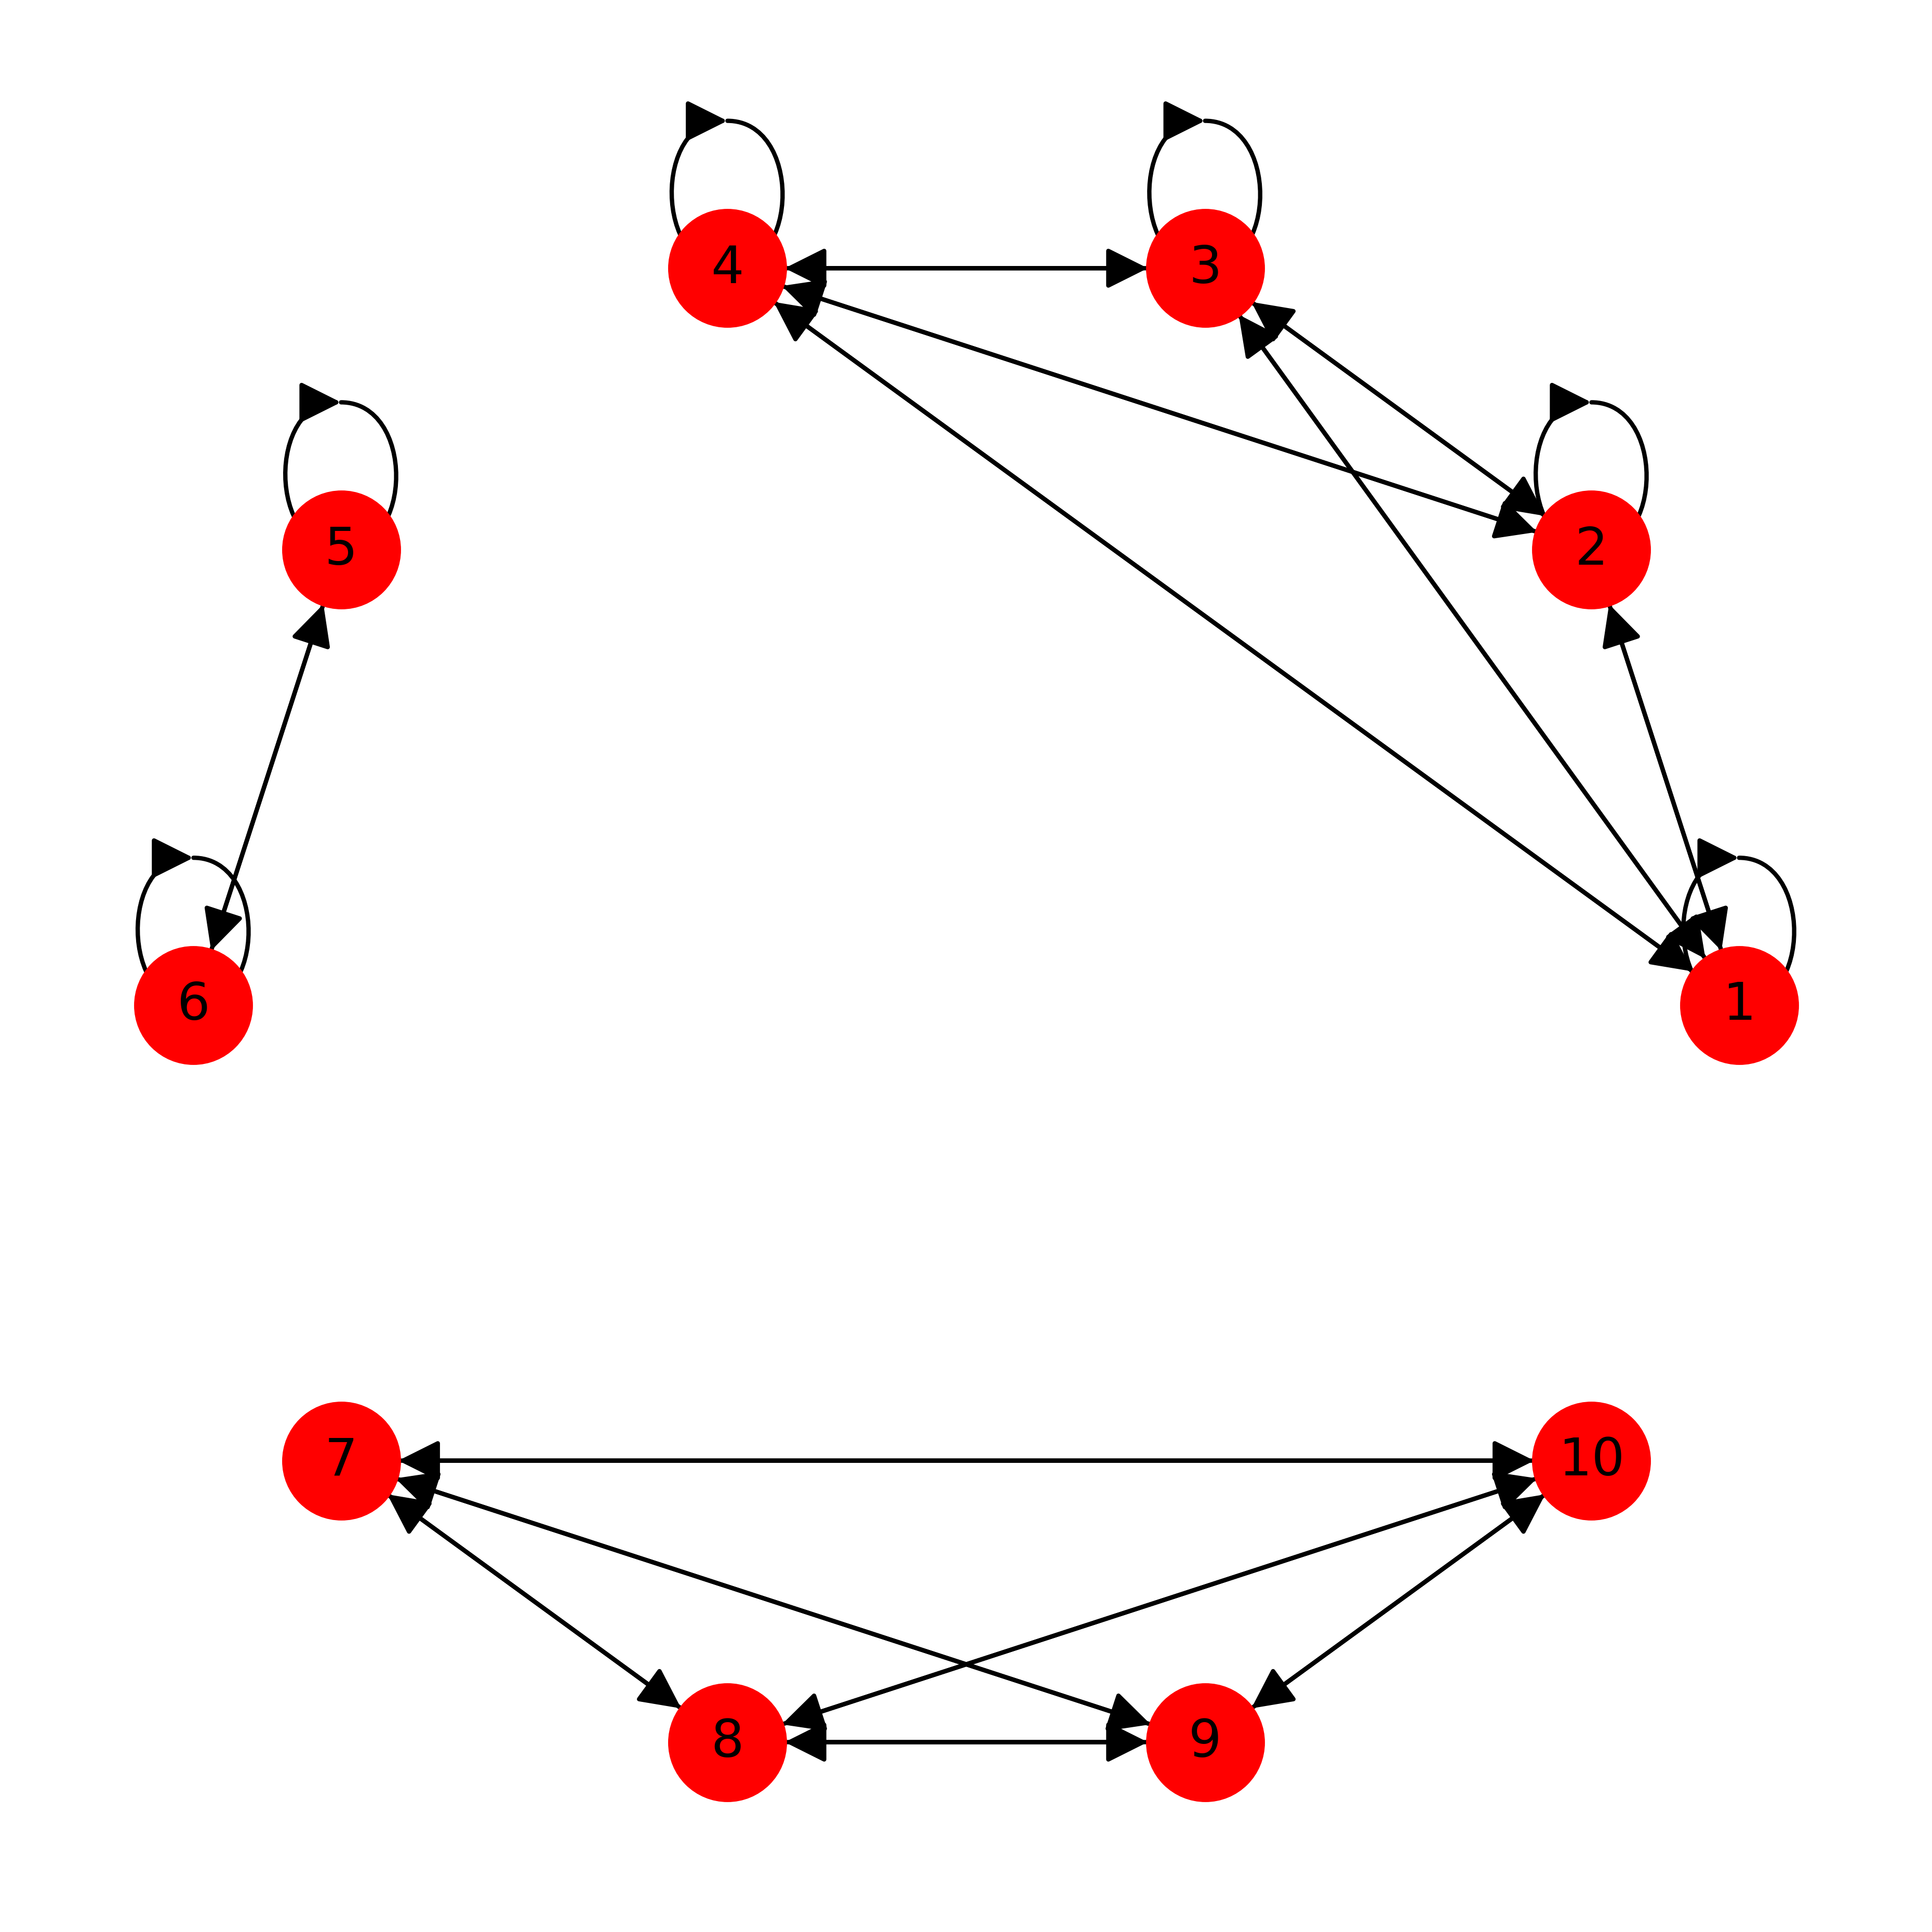
\includegraphics[width=0.4\linewidth]{img/2.png}
    \caption{Нерефлексивный, Транзитивный, Симметричный}
\end{figure}

\begin{figure}[h]
    \centering
    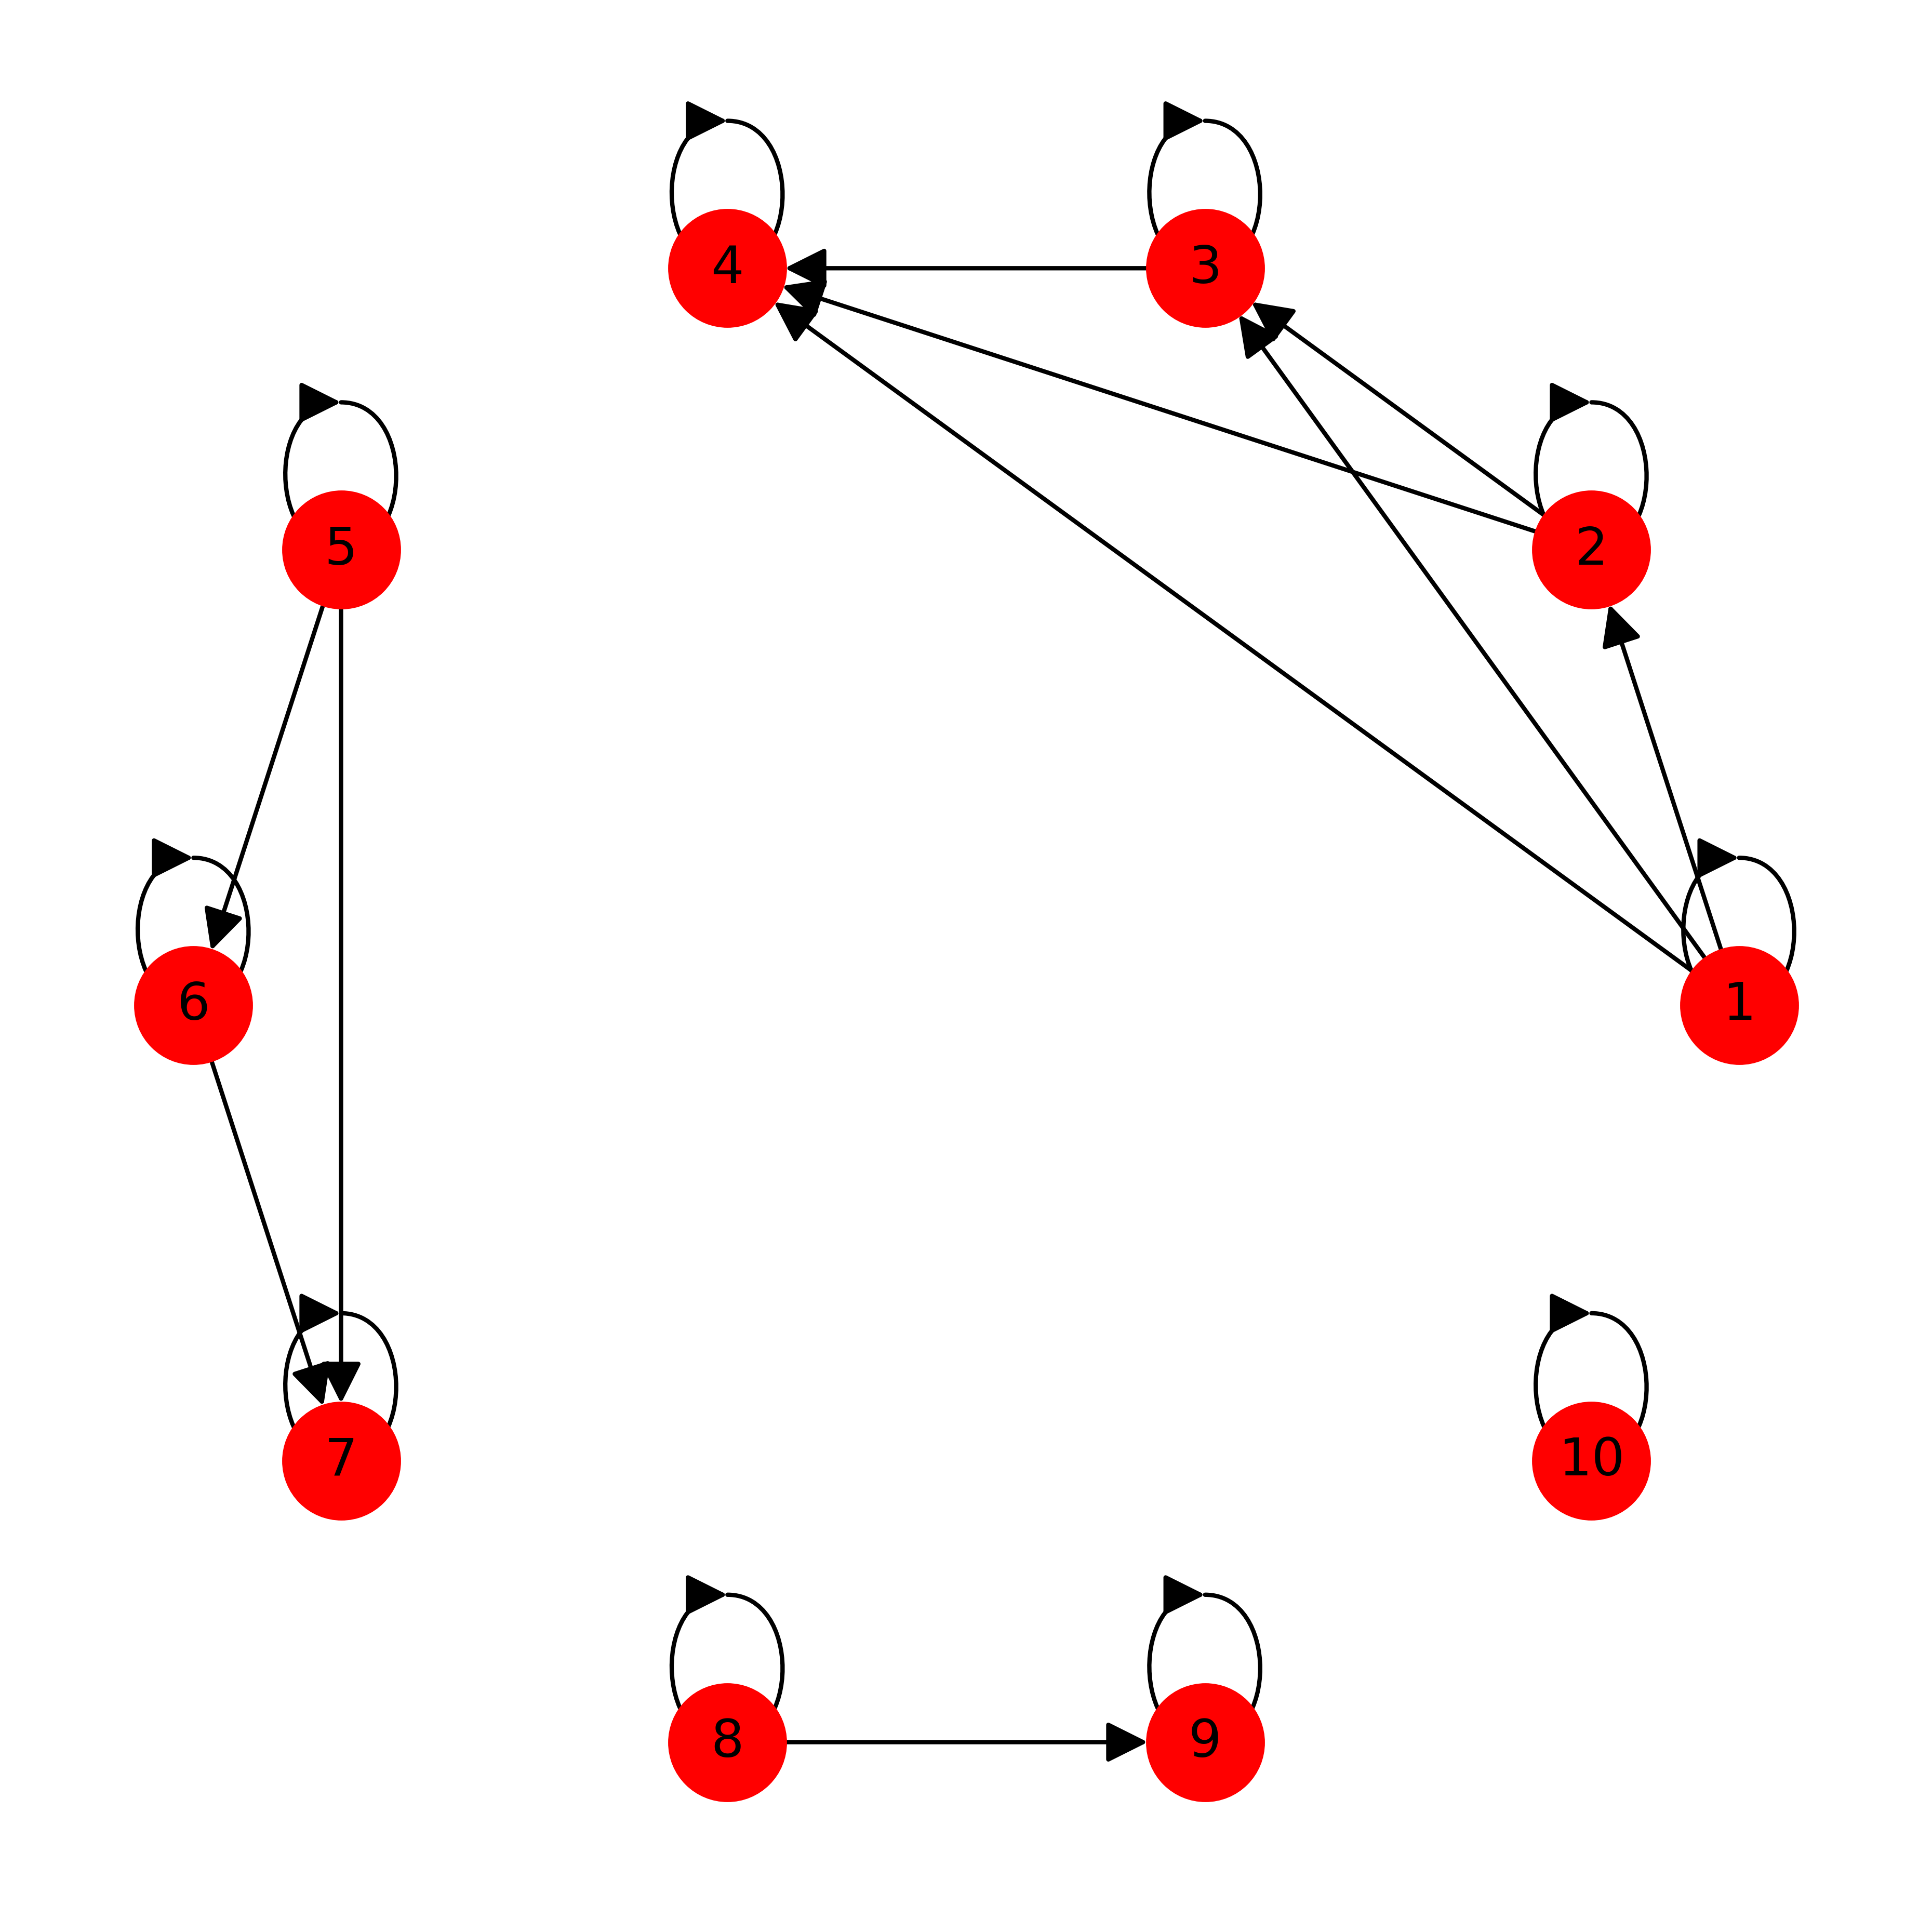
\includegraphics[width=0.4\linewidth]{img/3.png}
    \caption{Рефлексивный, Транзитивный, Несимметричный, Антисимметричный}
\end{figure}

\begin{figure}[h]
    \centering
    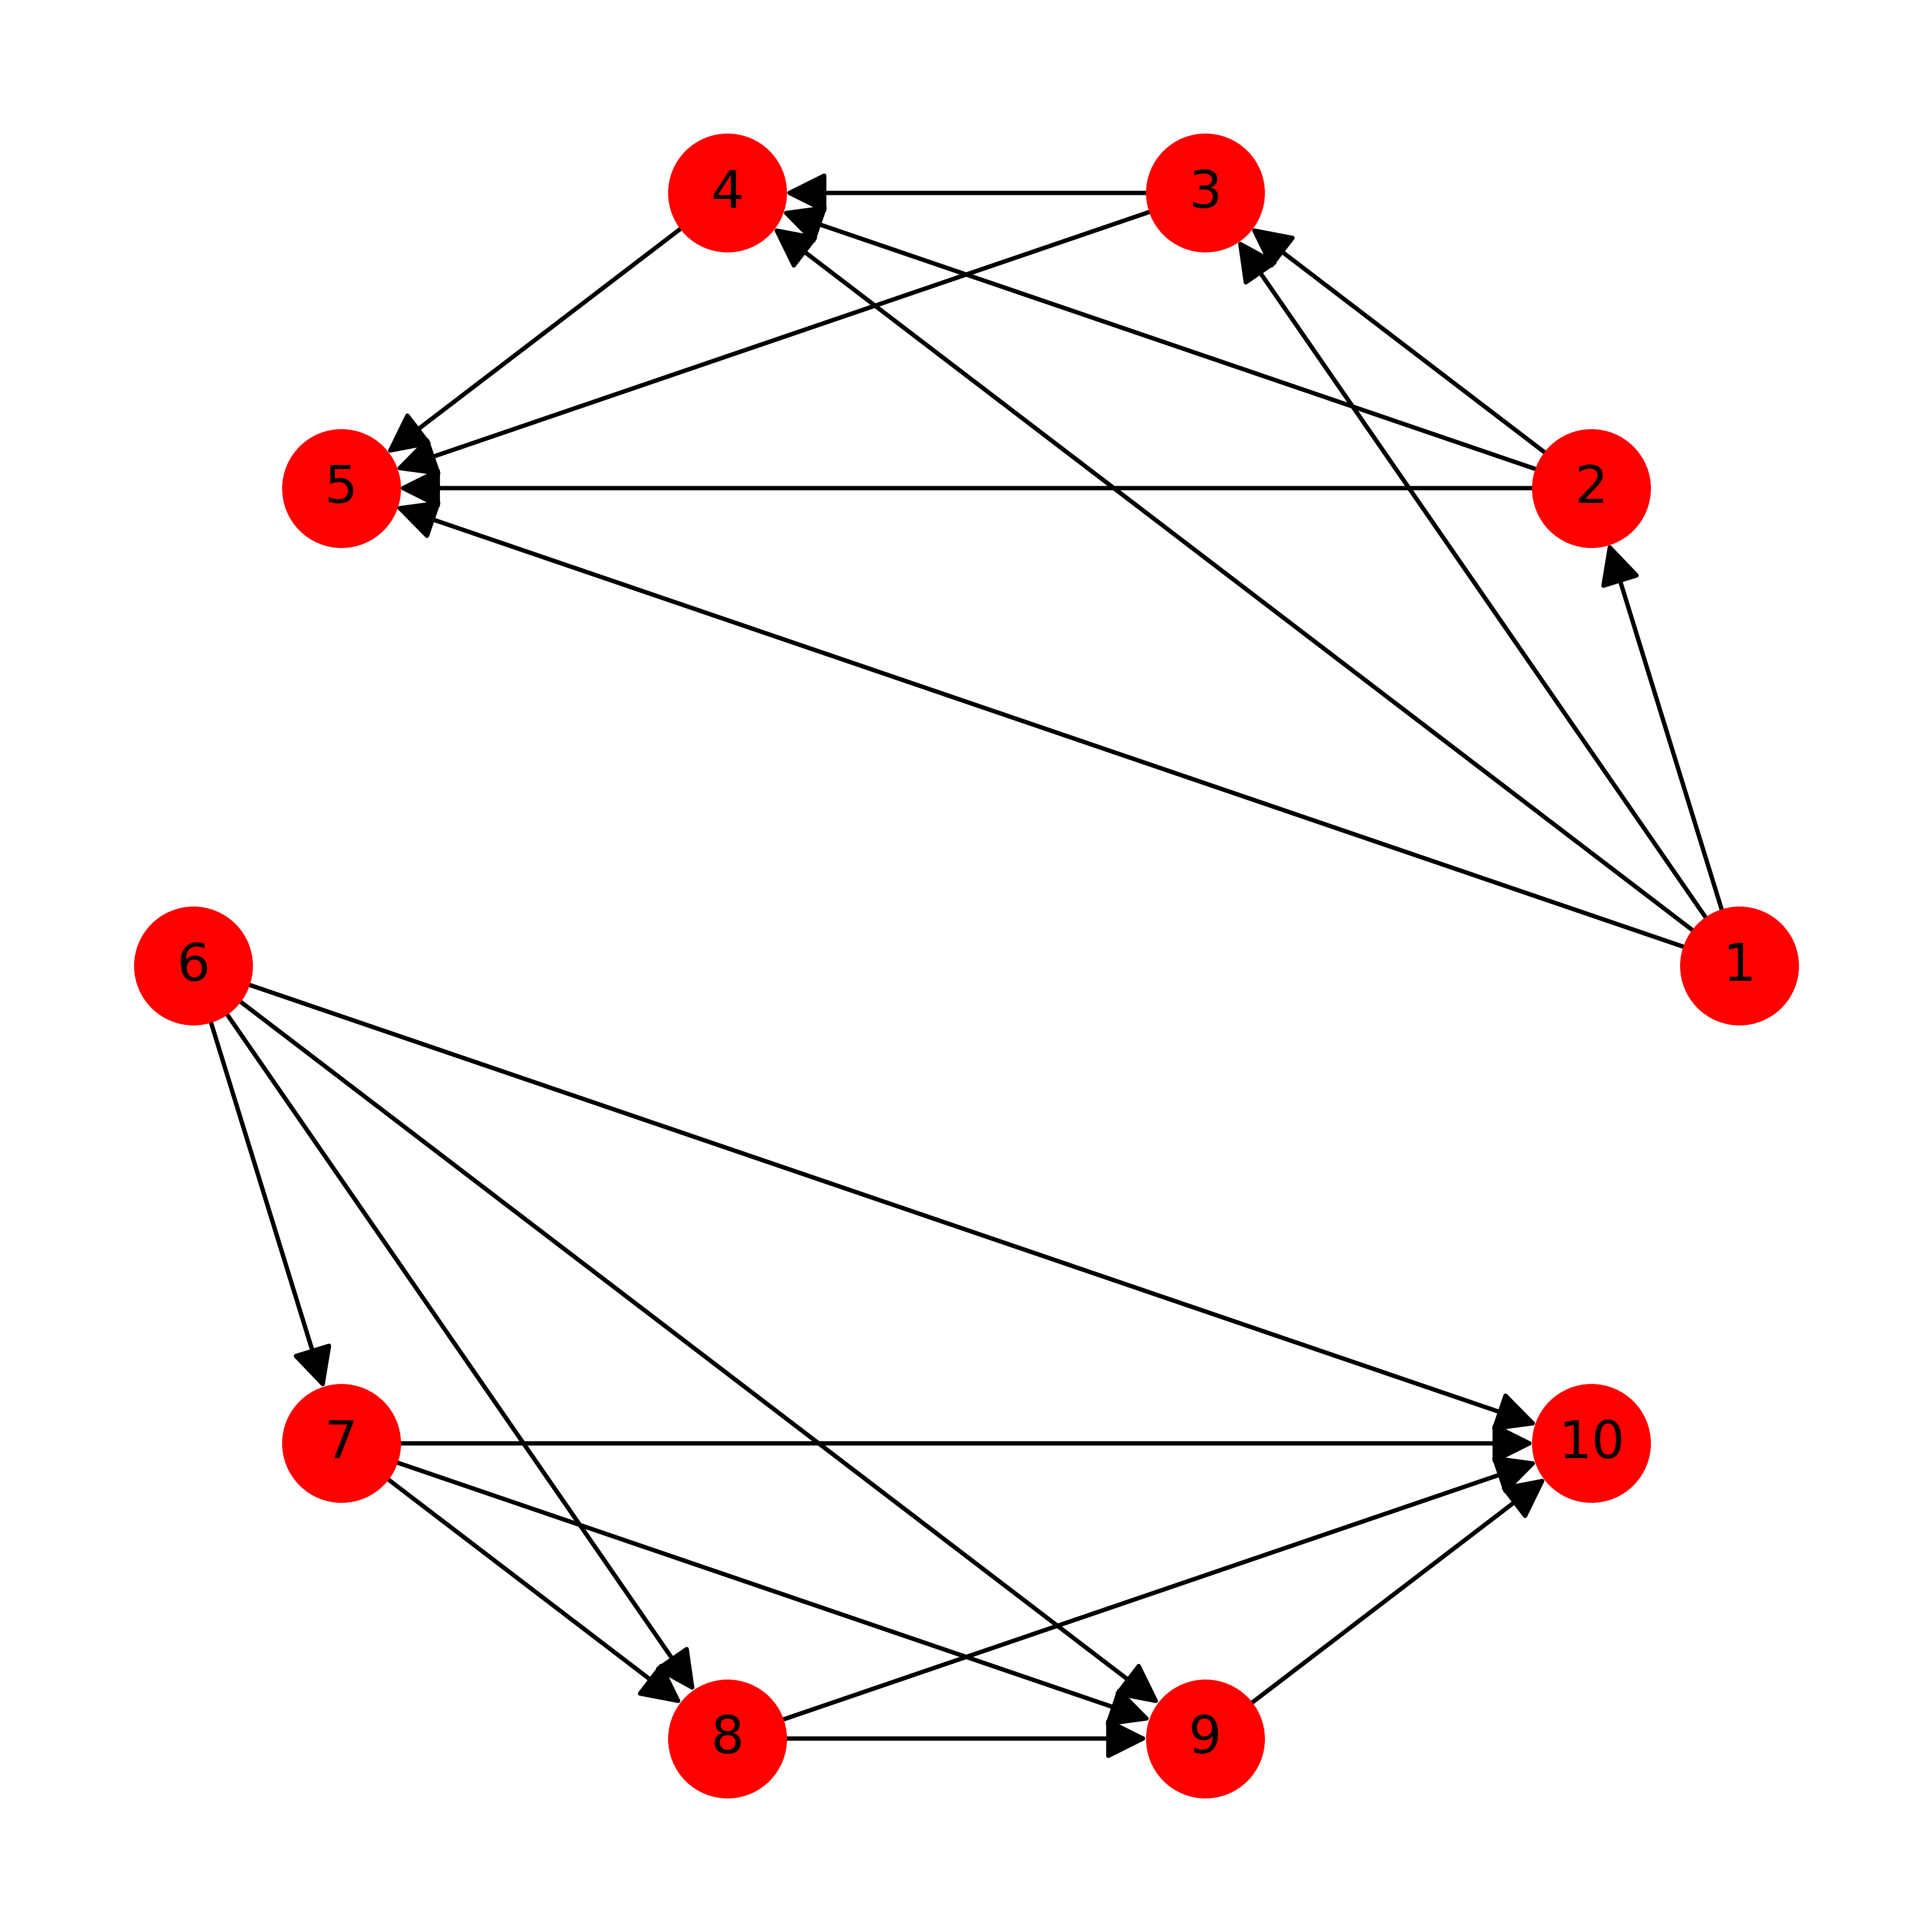
\includegraphics[width=0.4\linewidth]{img/4.png}
    \caption{Антирефлексивный, Транзитивный, Несимметричный, Антисимметричный}
\end{figure}

\begin{figure}[h]
    \centering
    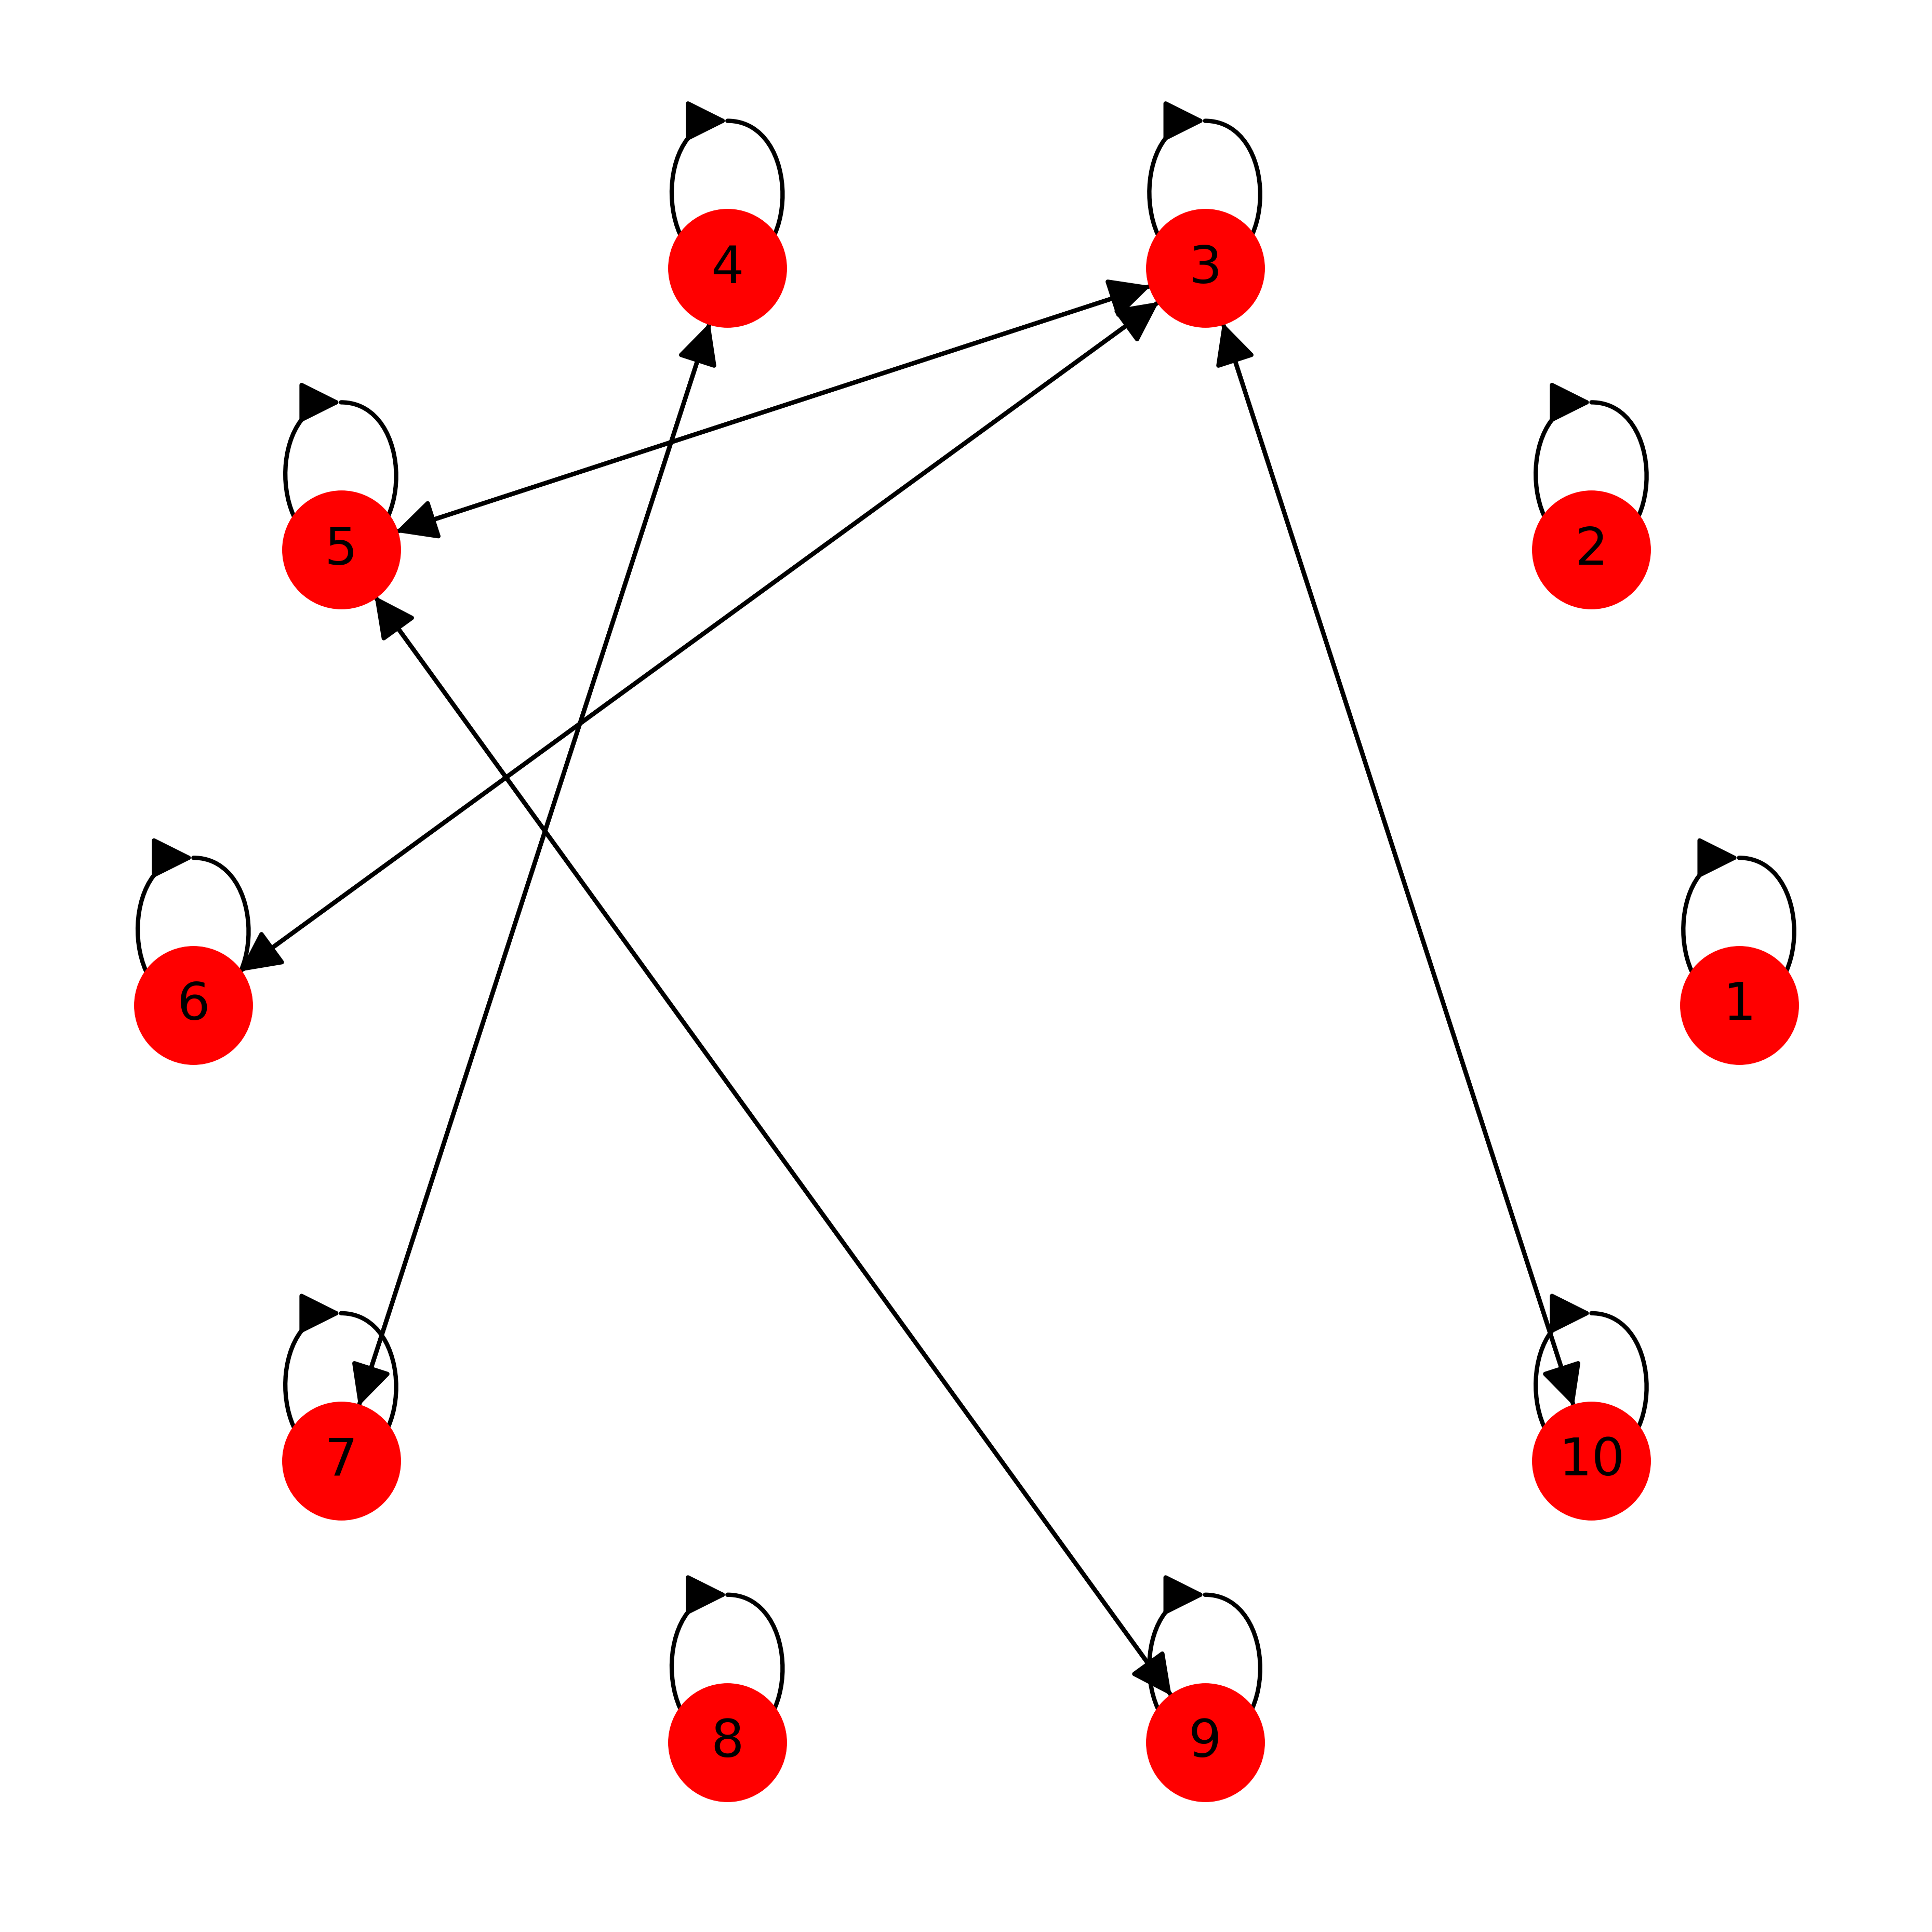
\includegraphics[width=0.4\linewidth]{img/5.png}
    \caption{Рефлексивный, Нетранзитивный, Симметричный}
\end{figure}

\begin{figure}[h]
    \centering
    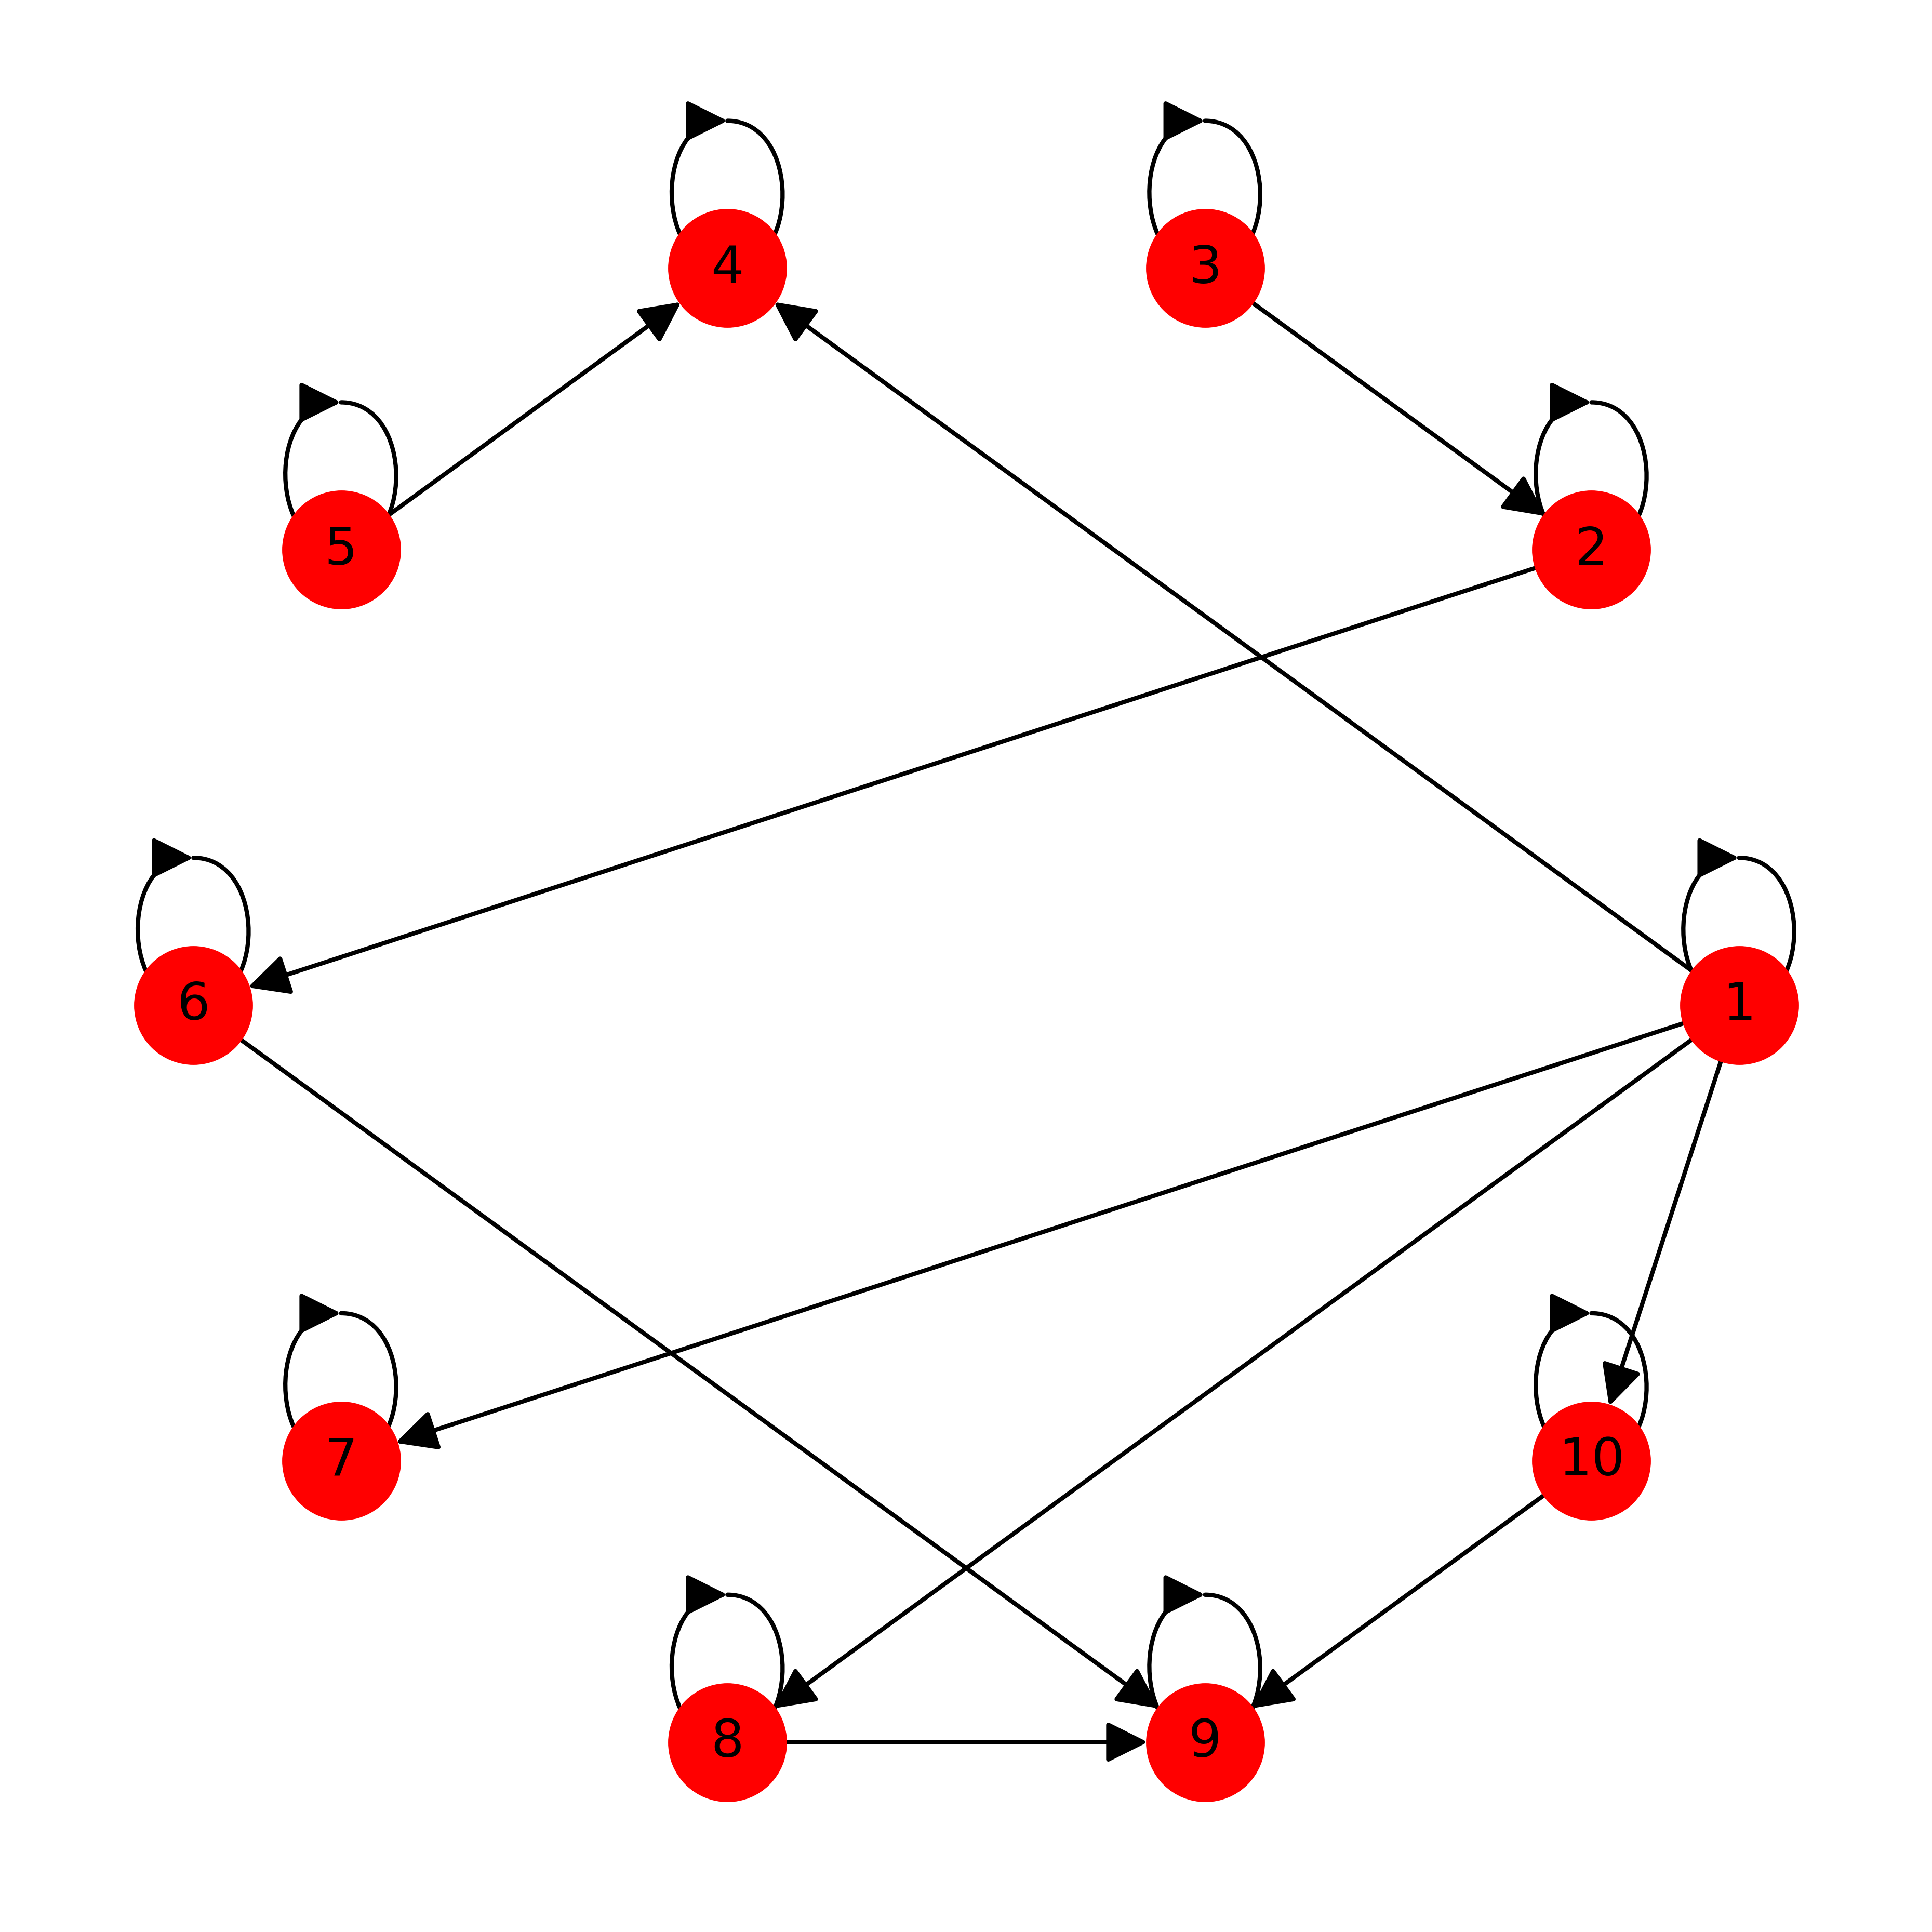
\includegraphics[width=0.4\linewidth]{img/6.png}
    \caption{Рефлексивный, Нетранзитивный, Несимметричный, Антисимметричный}
\end{figure}

\begin{figure}[h]
    \centering
    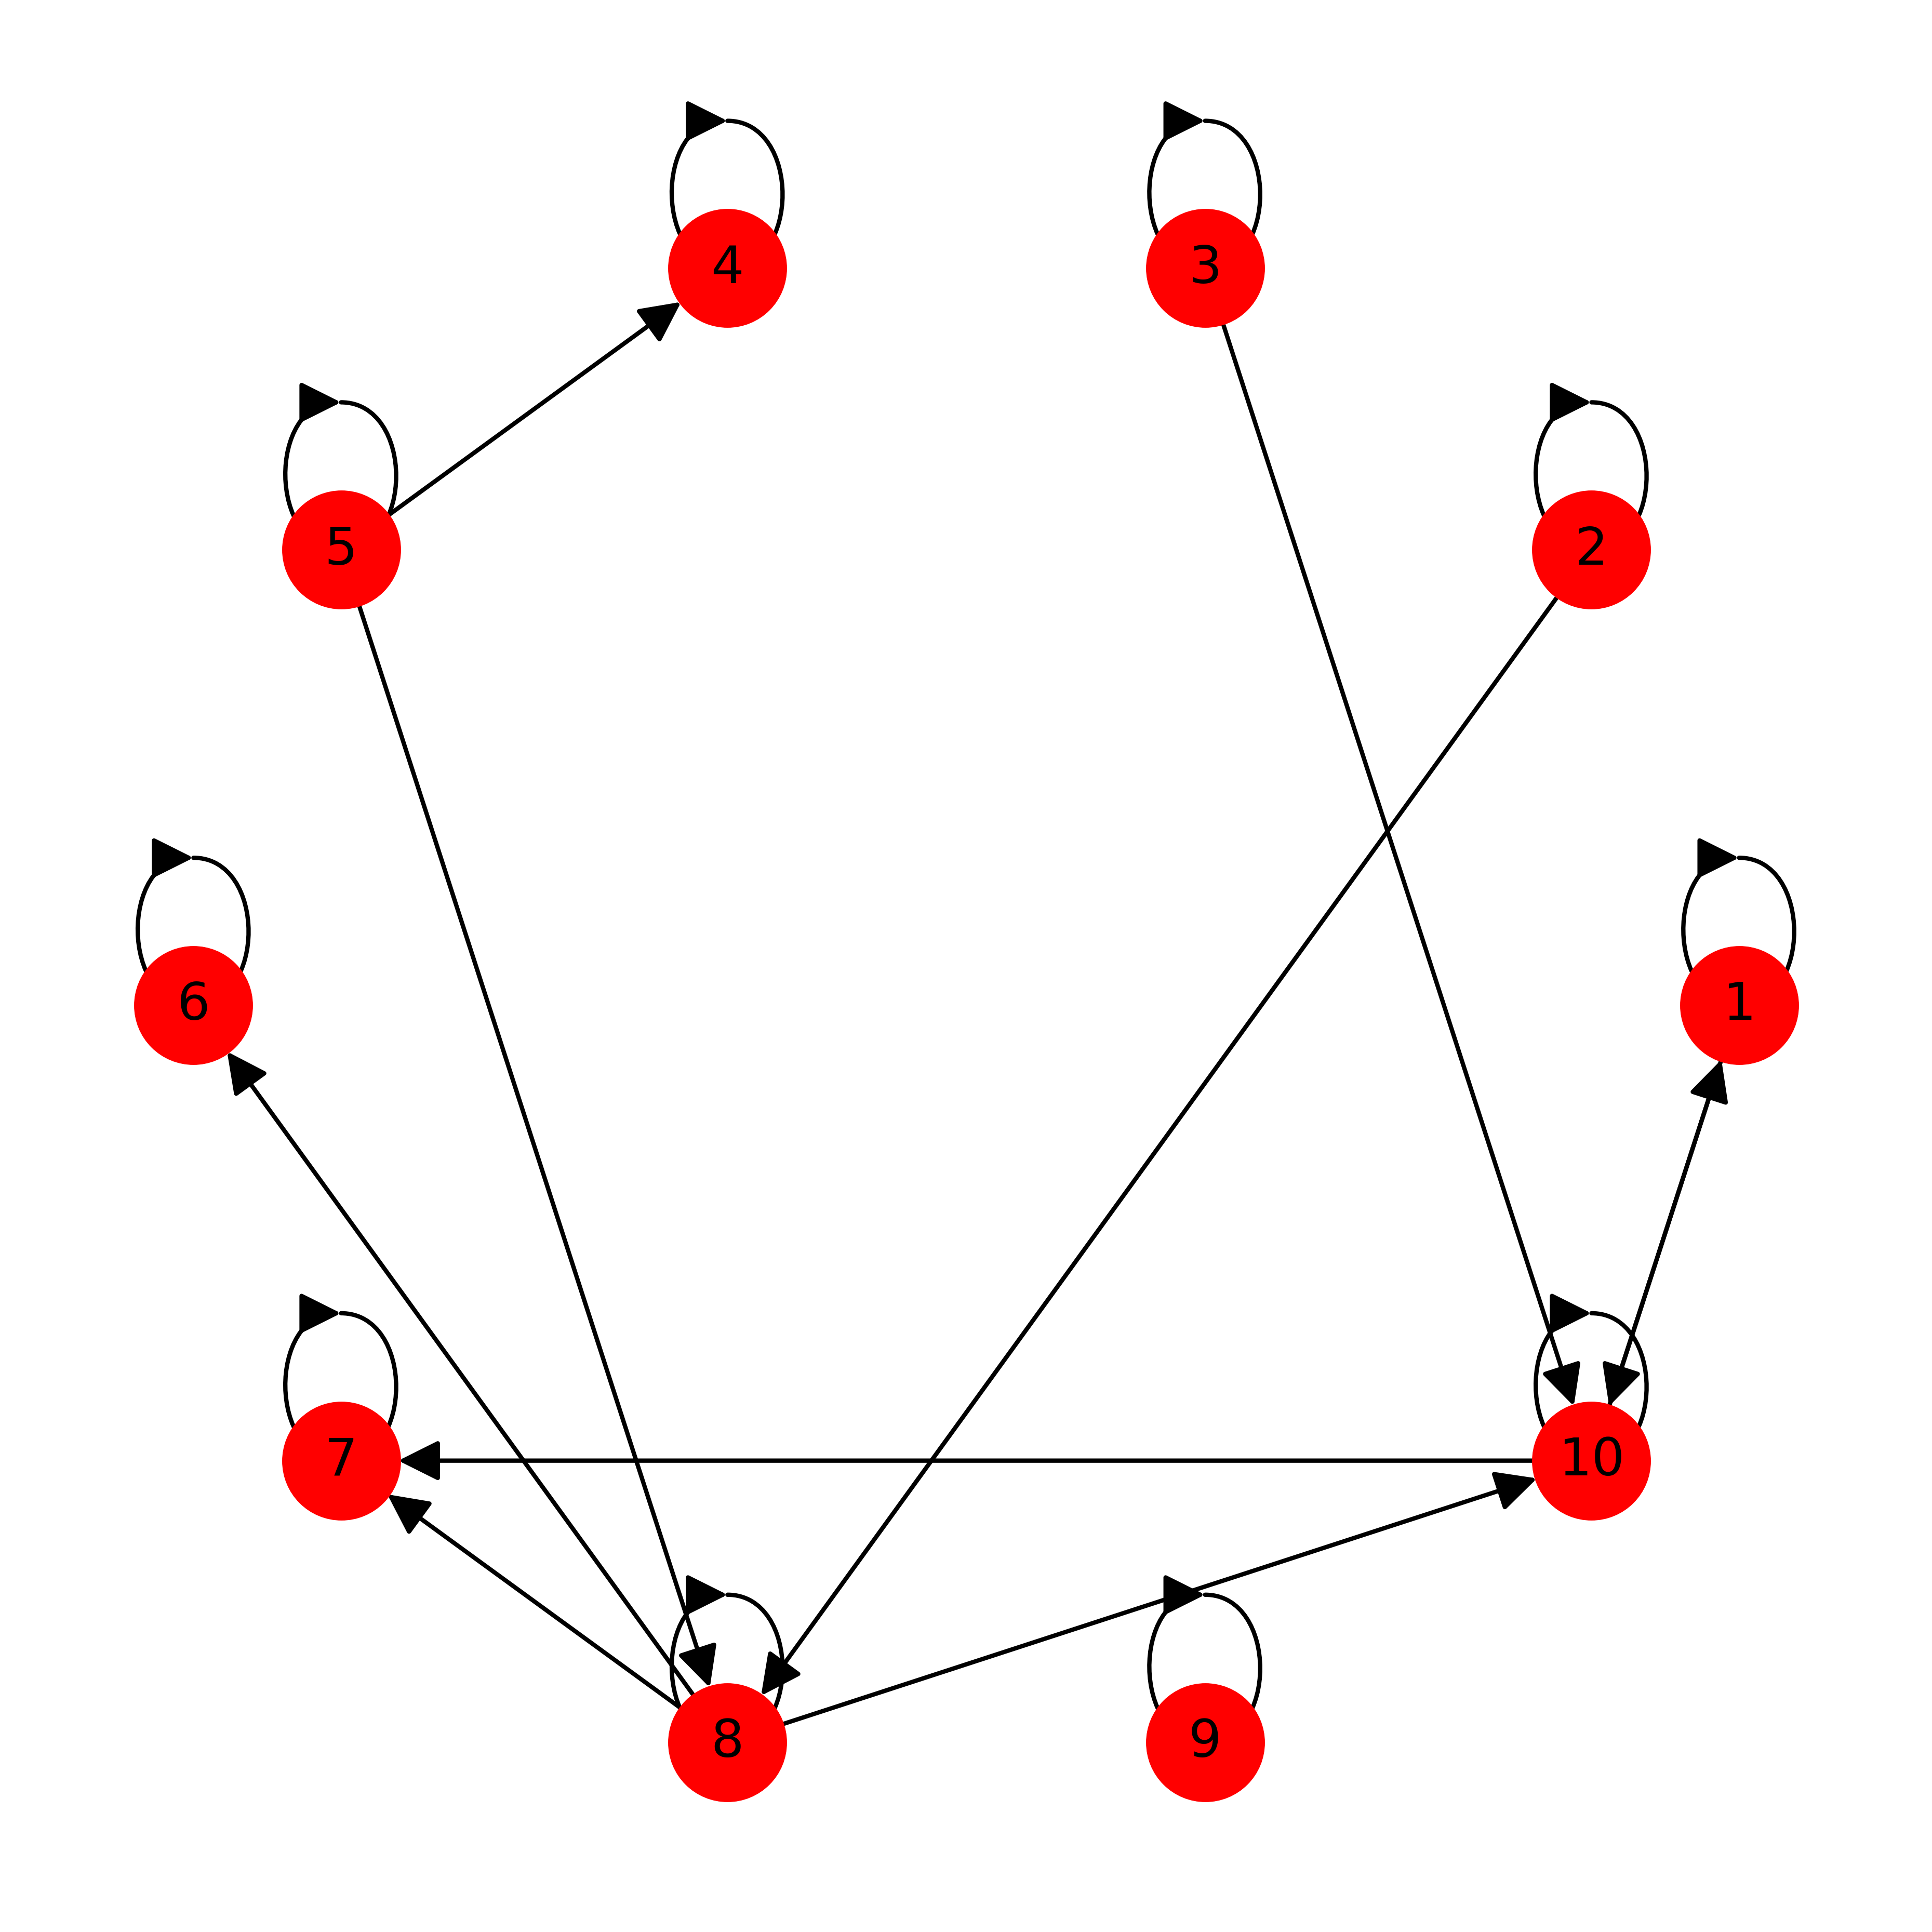
\includegraphics[width=0.4\linewidth]{img/7.png}
    \caption{Рефлексивный, Нетранзитивный, Несимметричный}
\end{figure}

\begin{figure}[h]
    \centering
    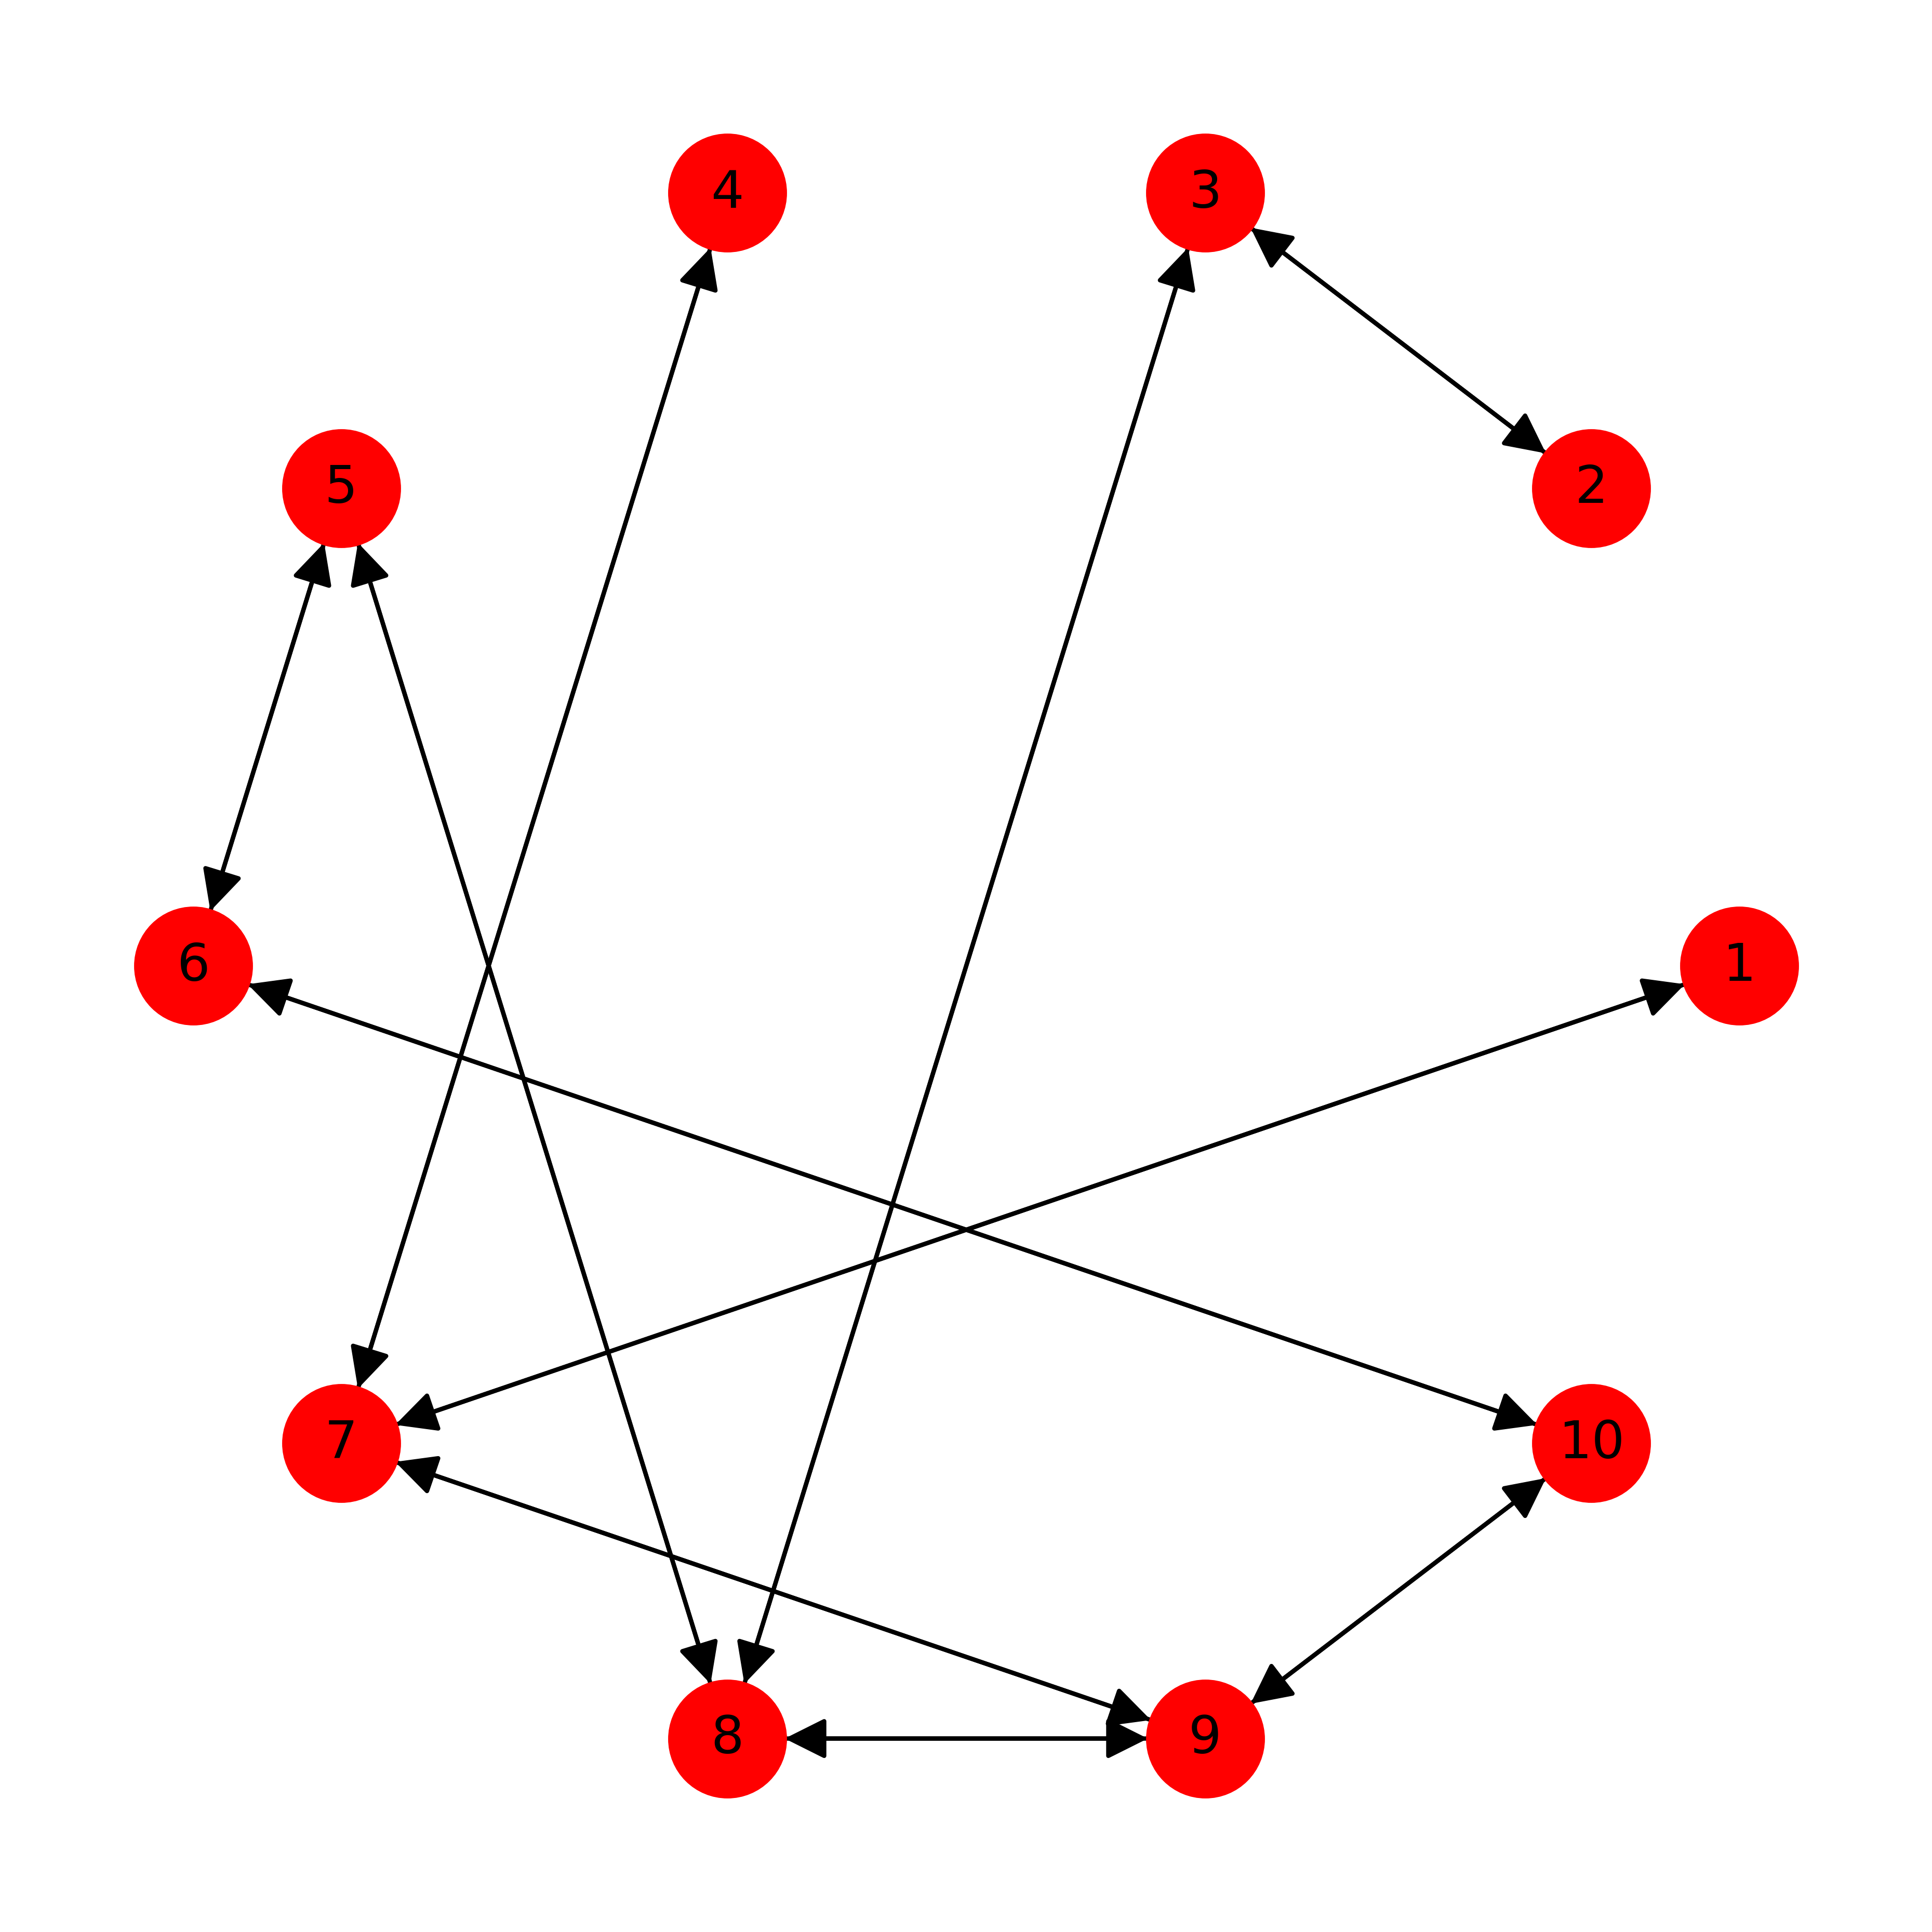
\includegraphics[width=0.4\linewidth]{img/8.png}
    \caption{Антирефлексивный, Нетранзитивный, Симметричный}
\end{figure}

\begin{figure}[h]
    \centering
    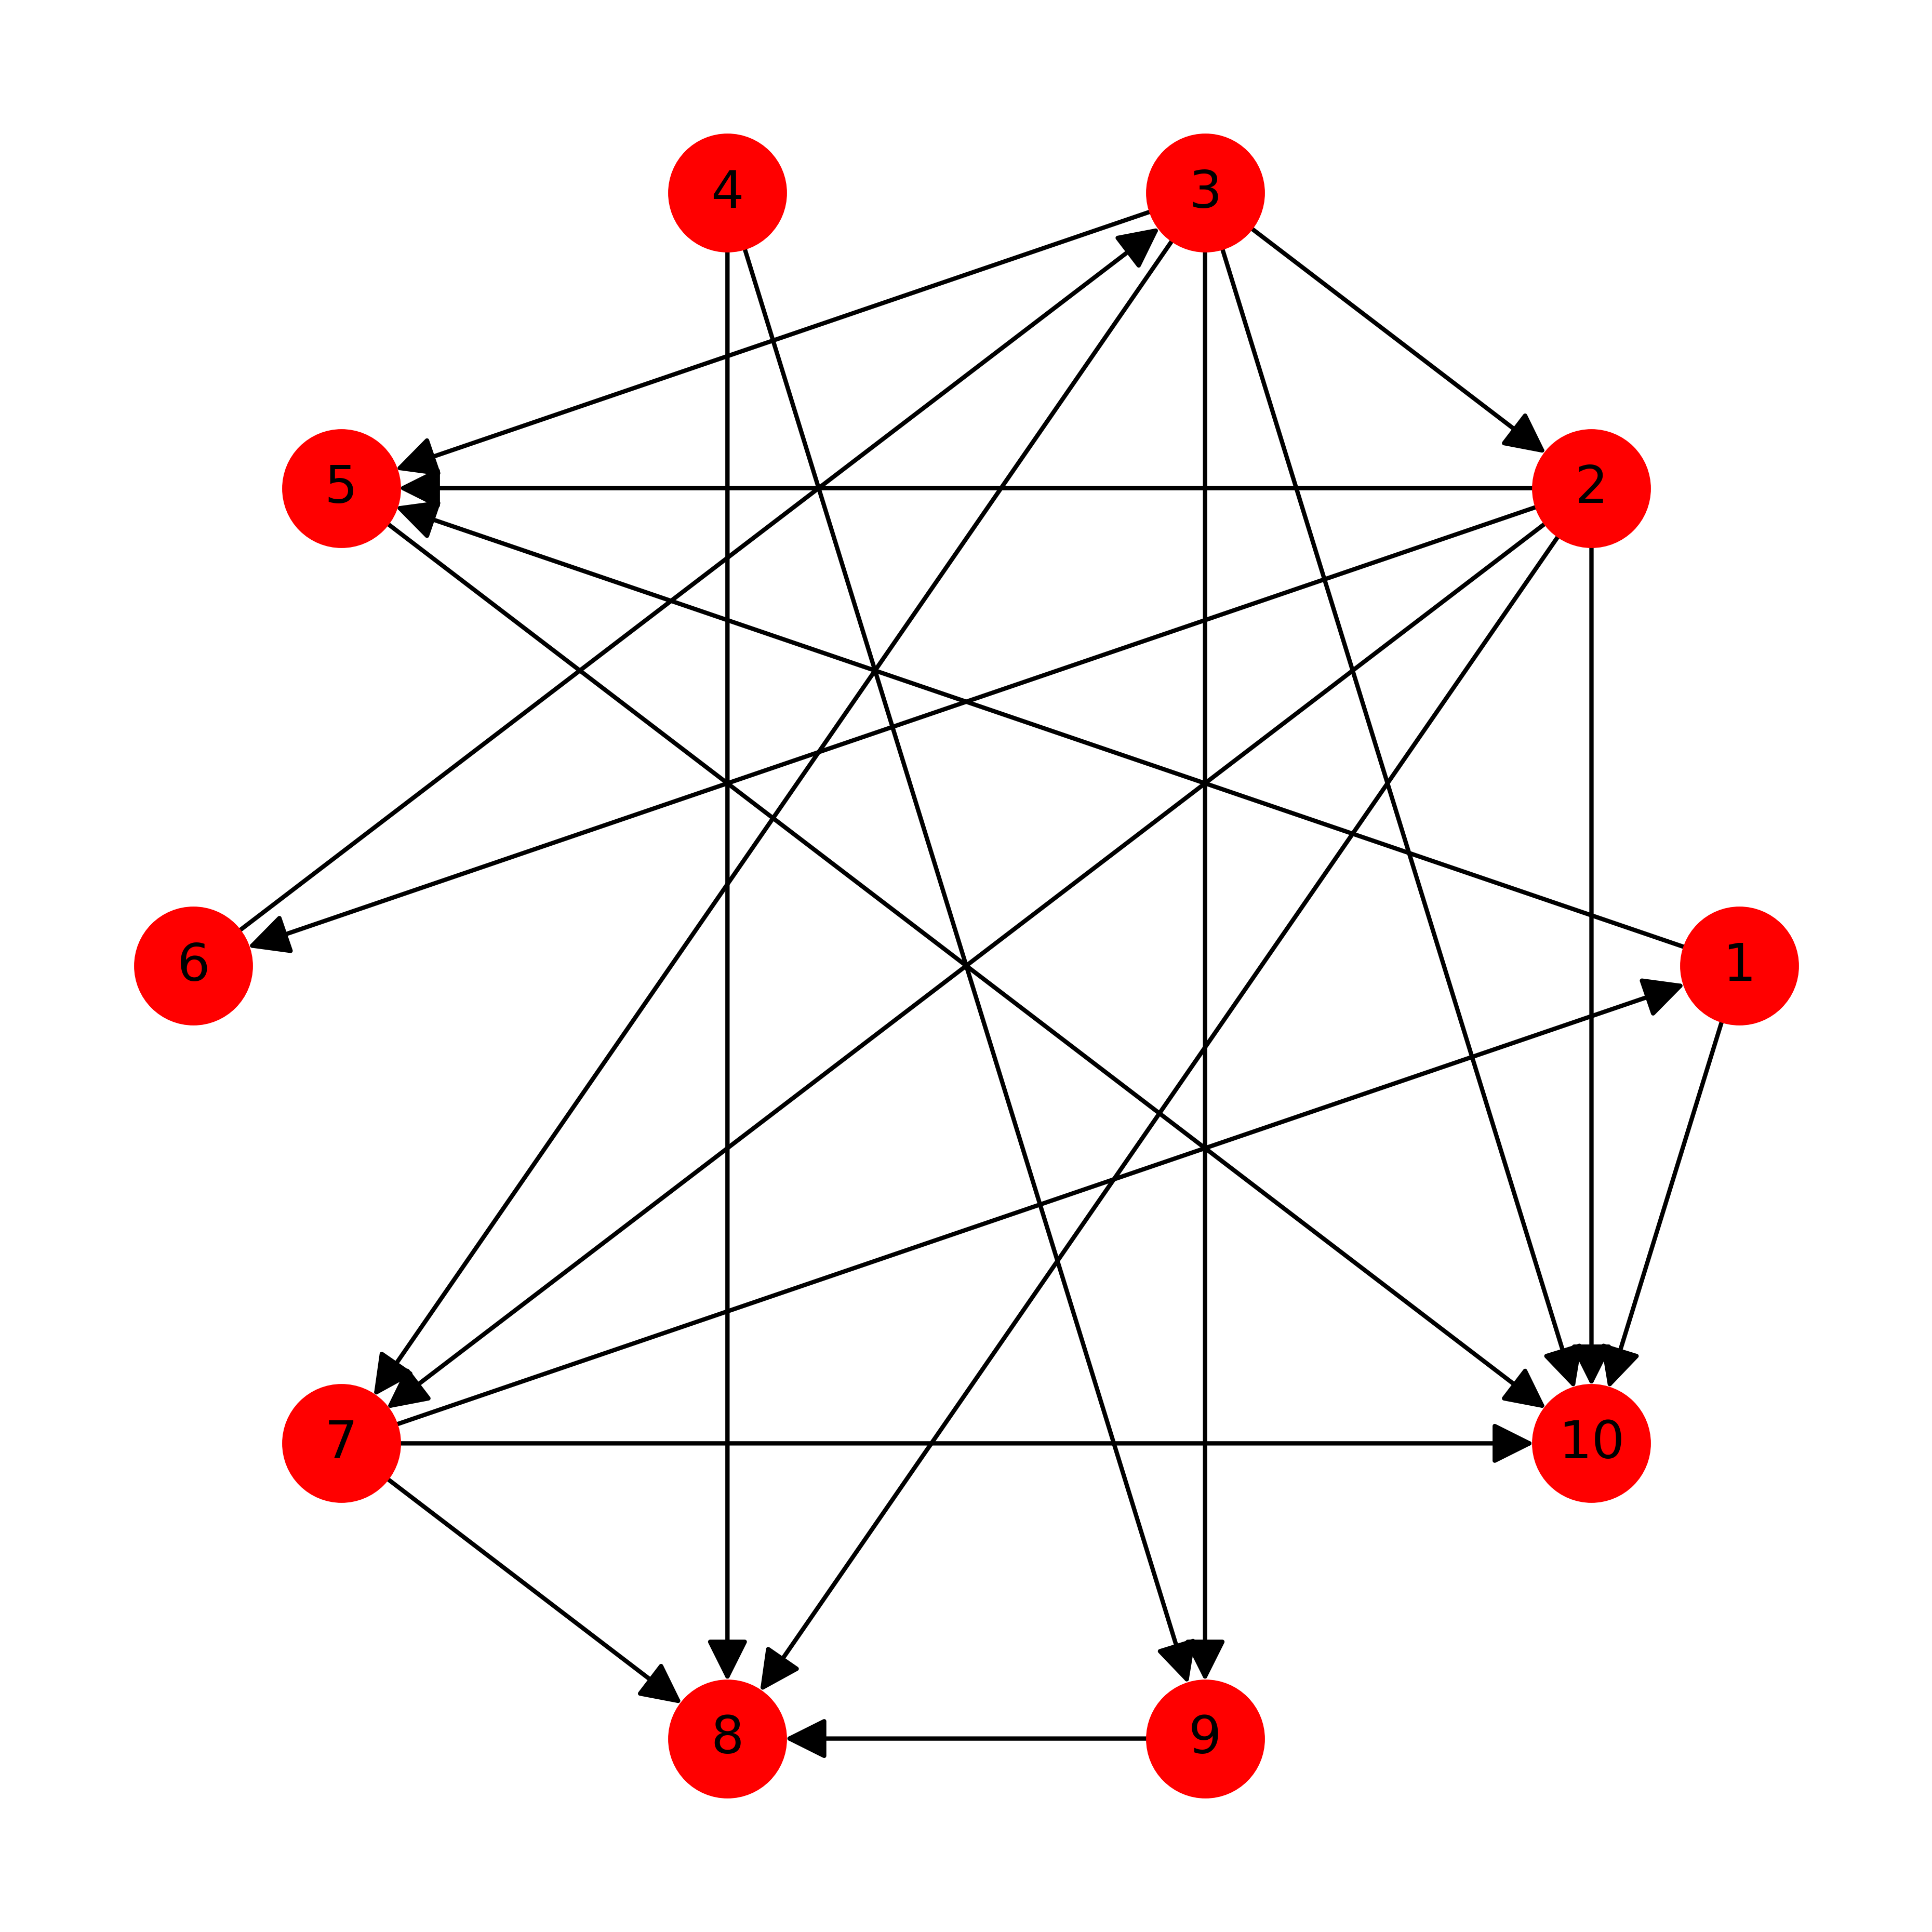
\includegraphics[width=0.4\linewidth]{img/9.png}
    \caption{Антирефлексивный, Нетранзитивный, Несимметричный, Антисимметричный}
\end{figure}

\begin{figure}[h]
    \centering
    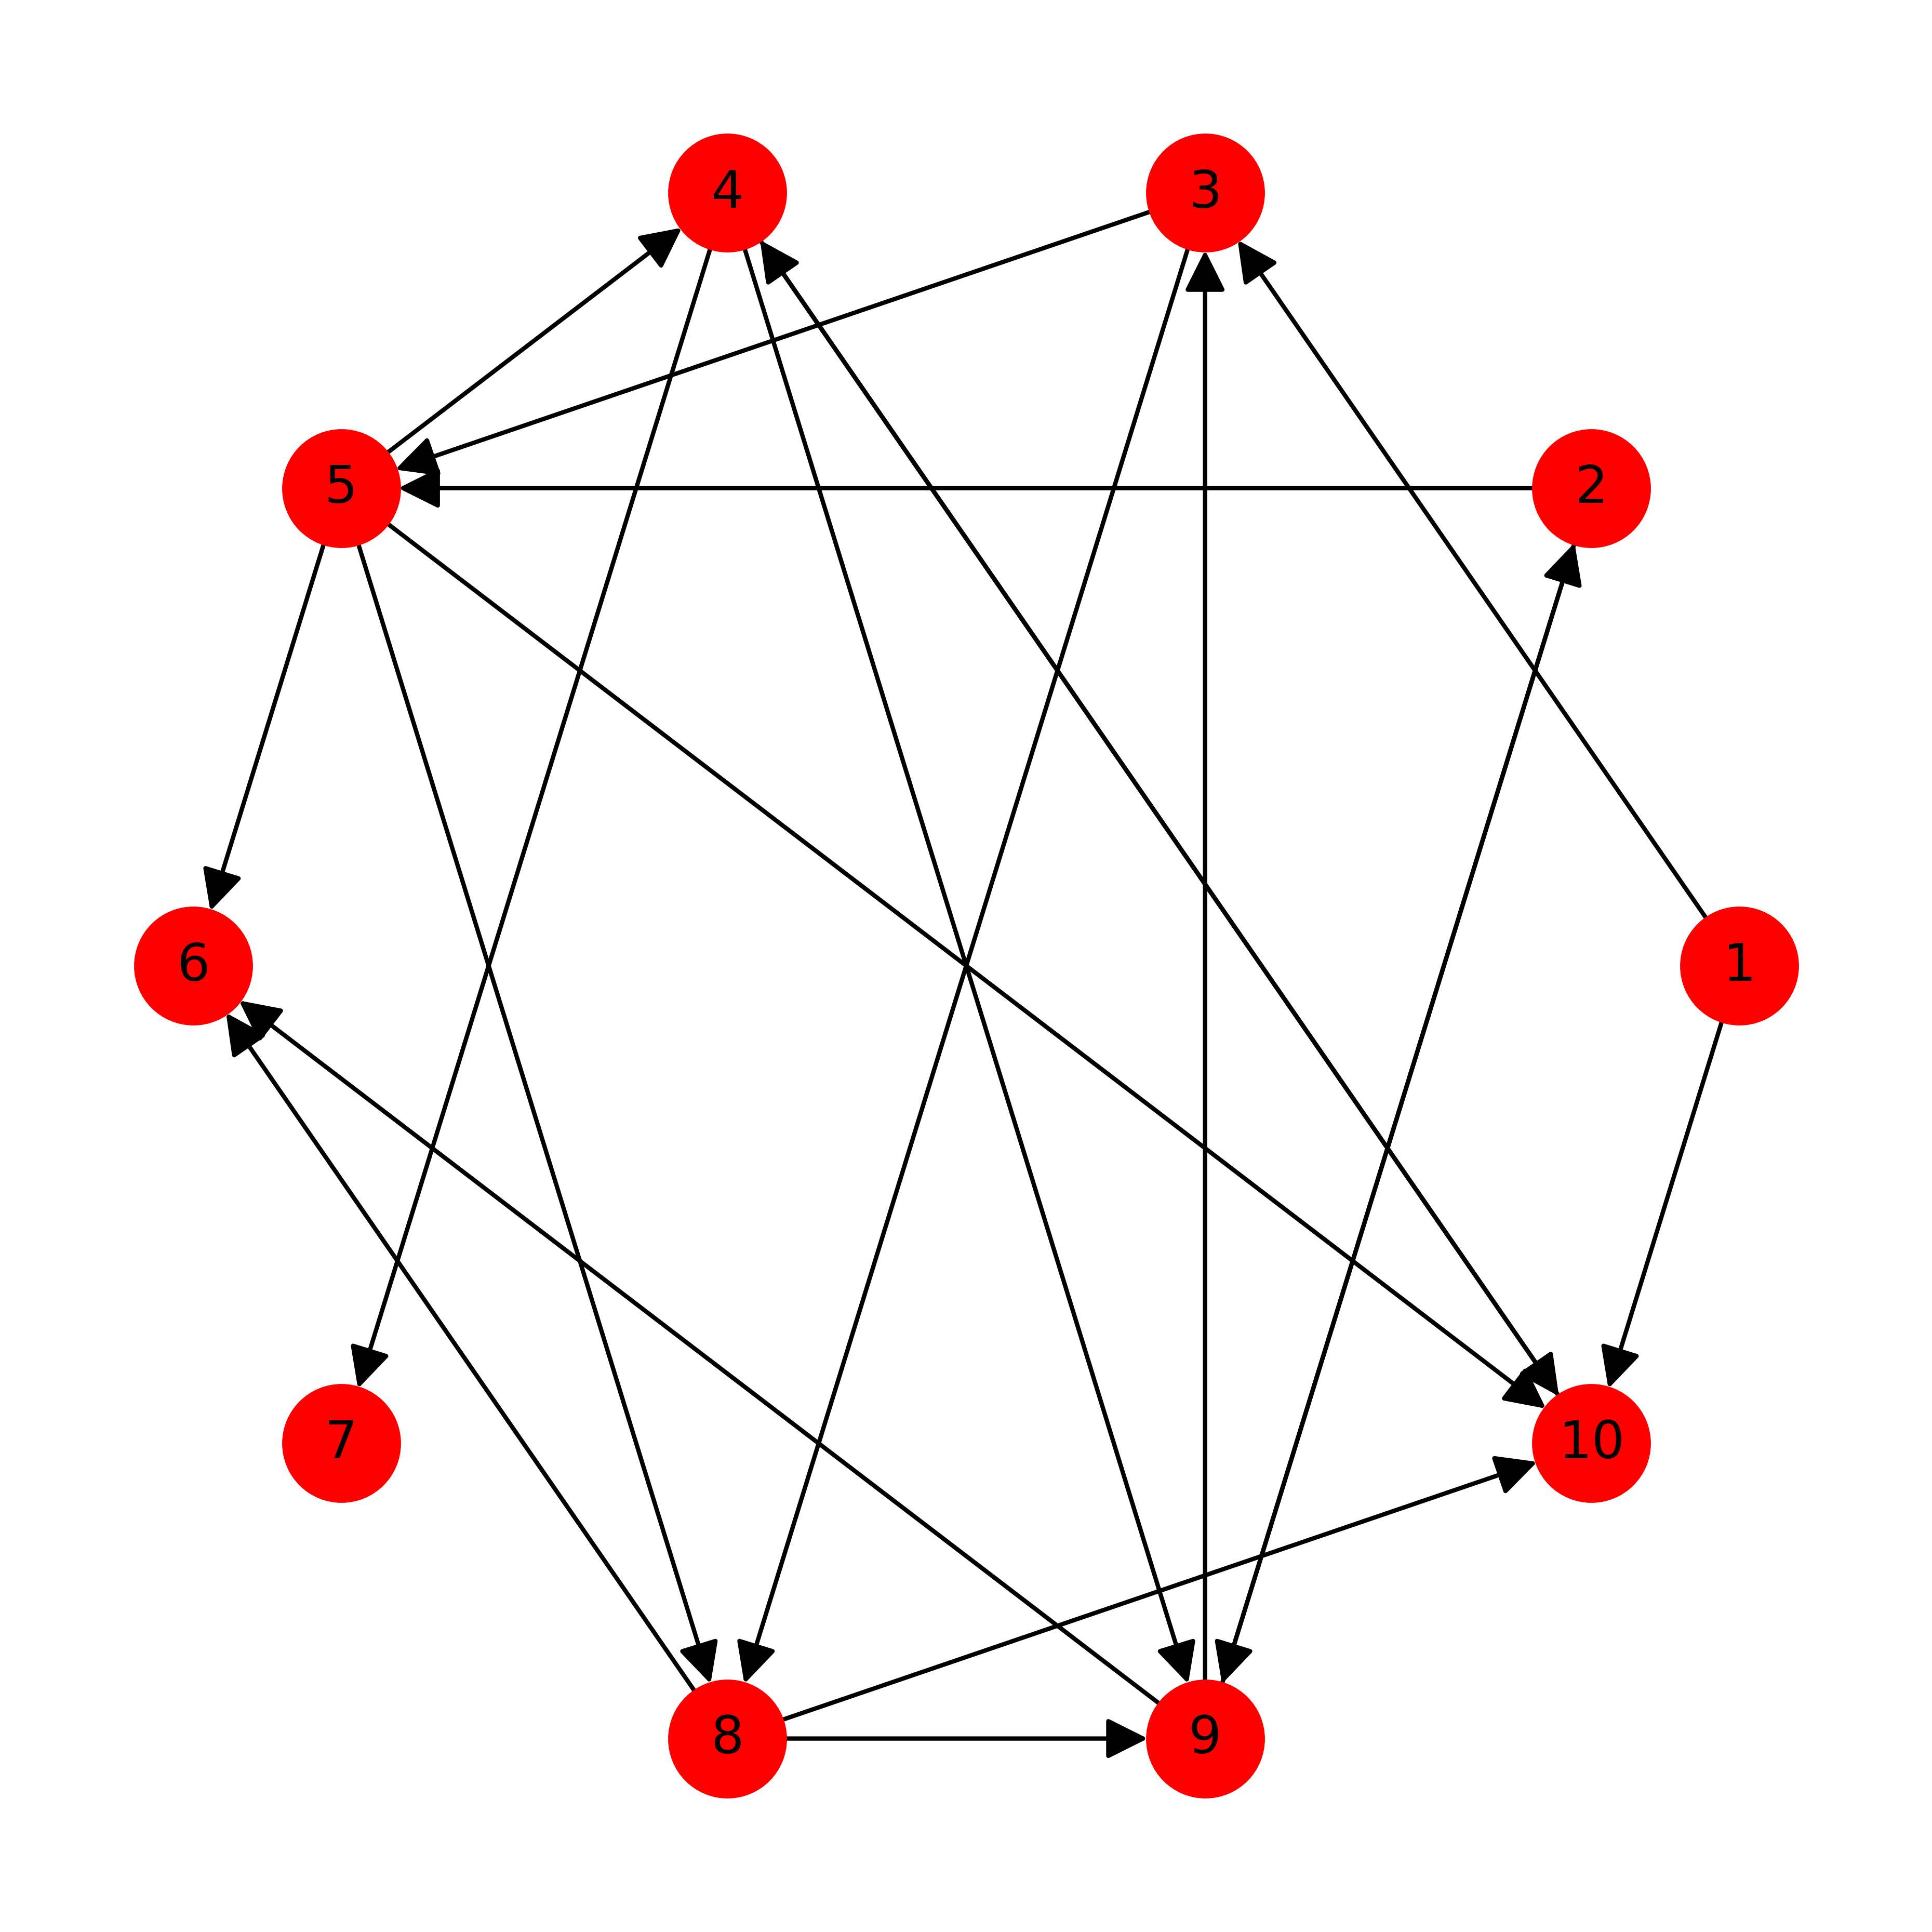
\includegraphics[width=0.4\linewidth]{img/10.png}
    \caption{Антирефлексивный, Нетранзитивный, Несимметричный}
\end{figure}

\begin{figure}[h]
    \centering
    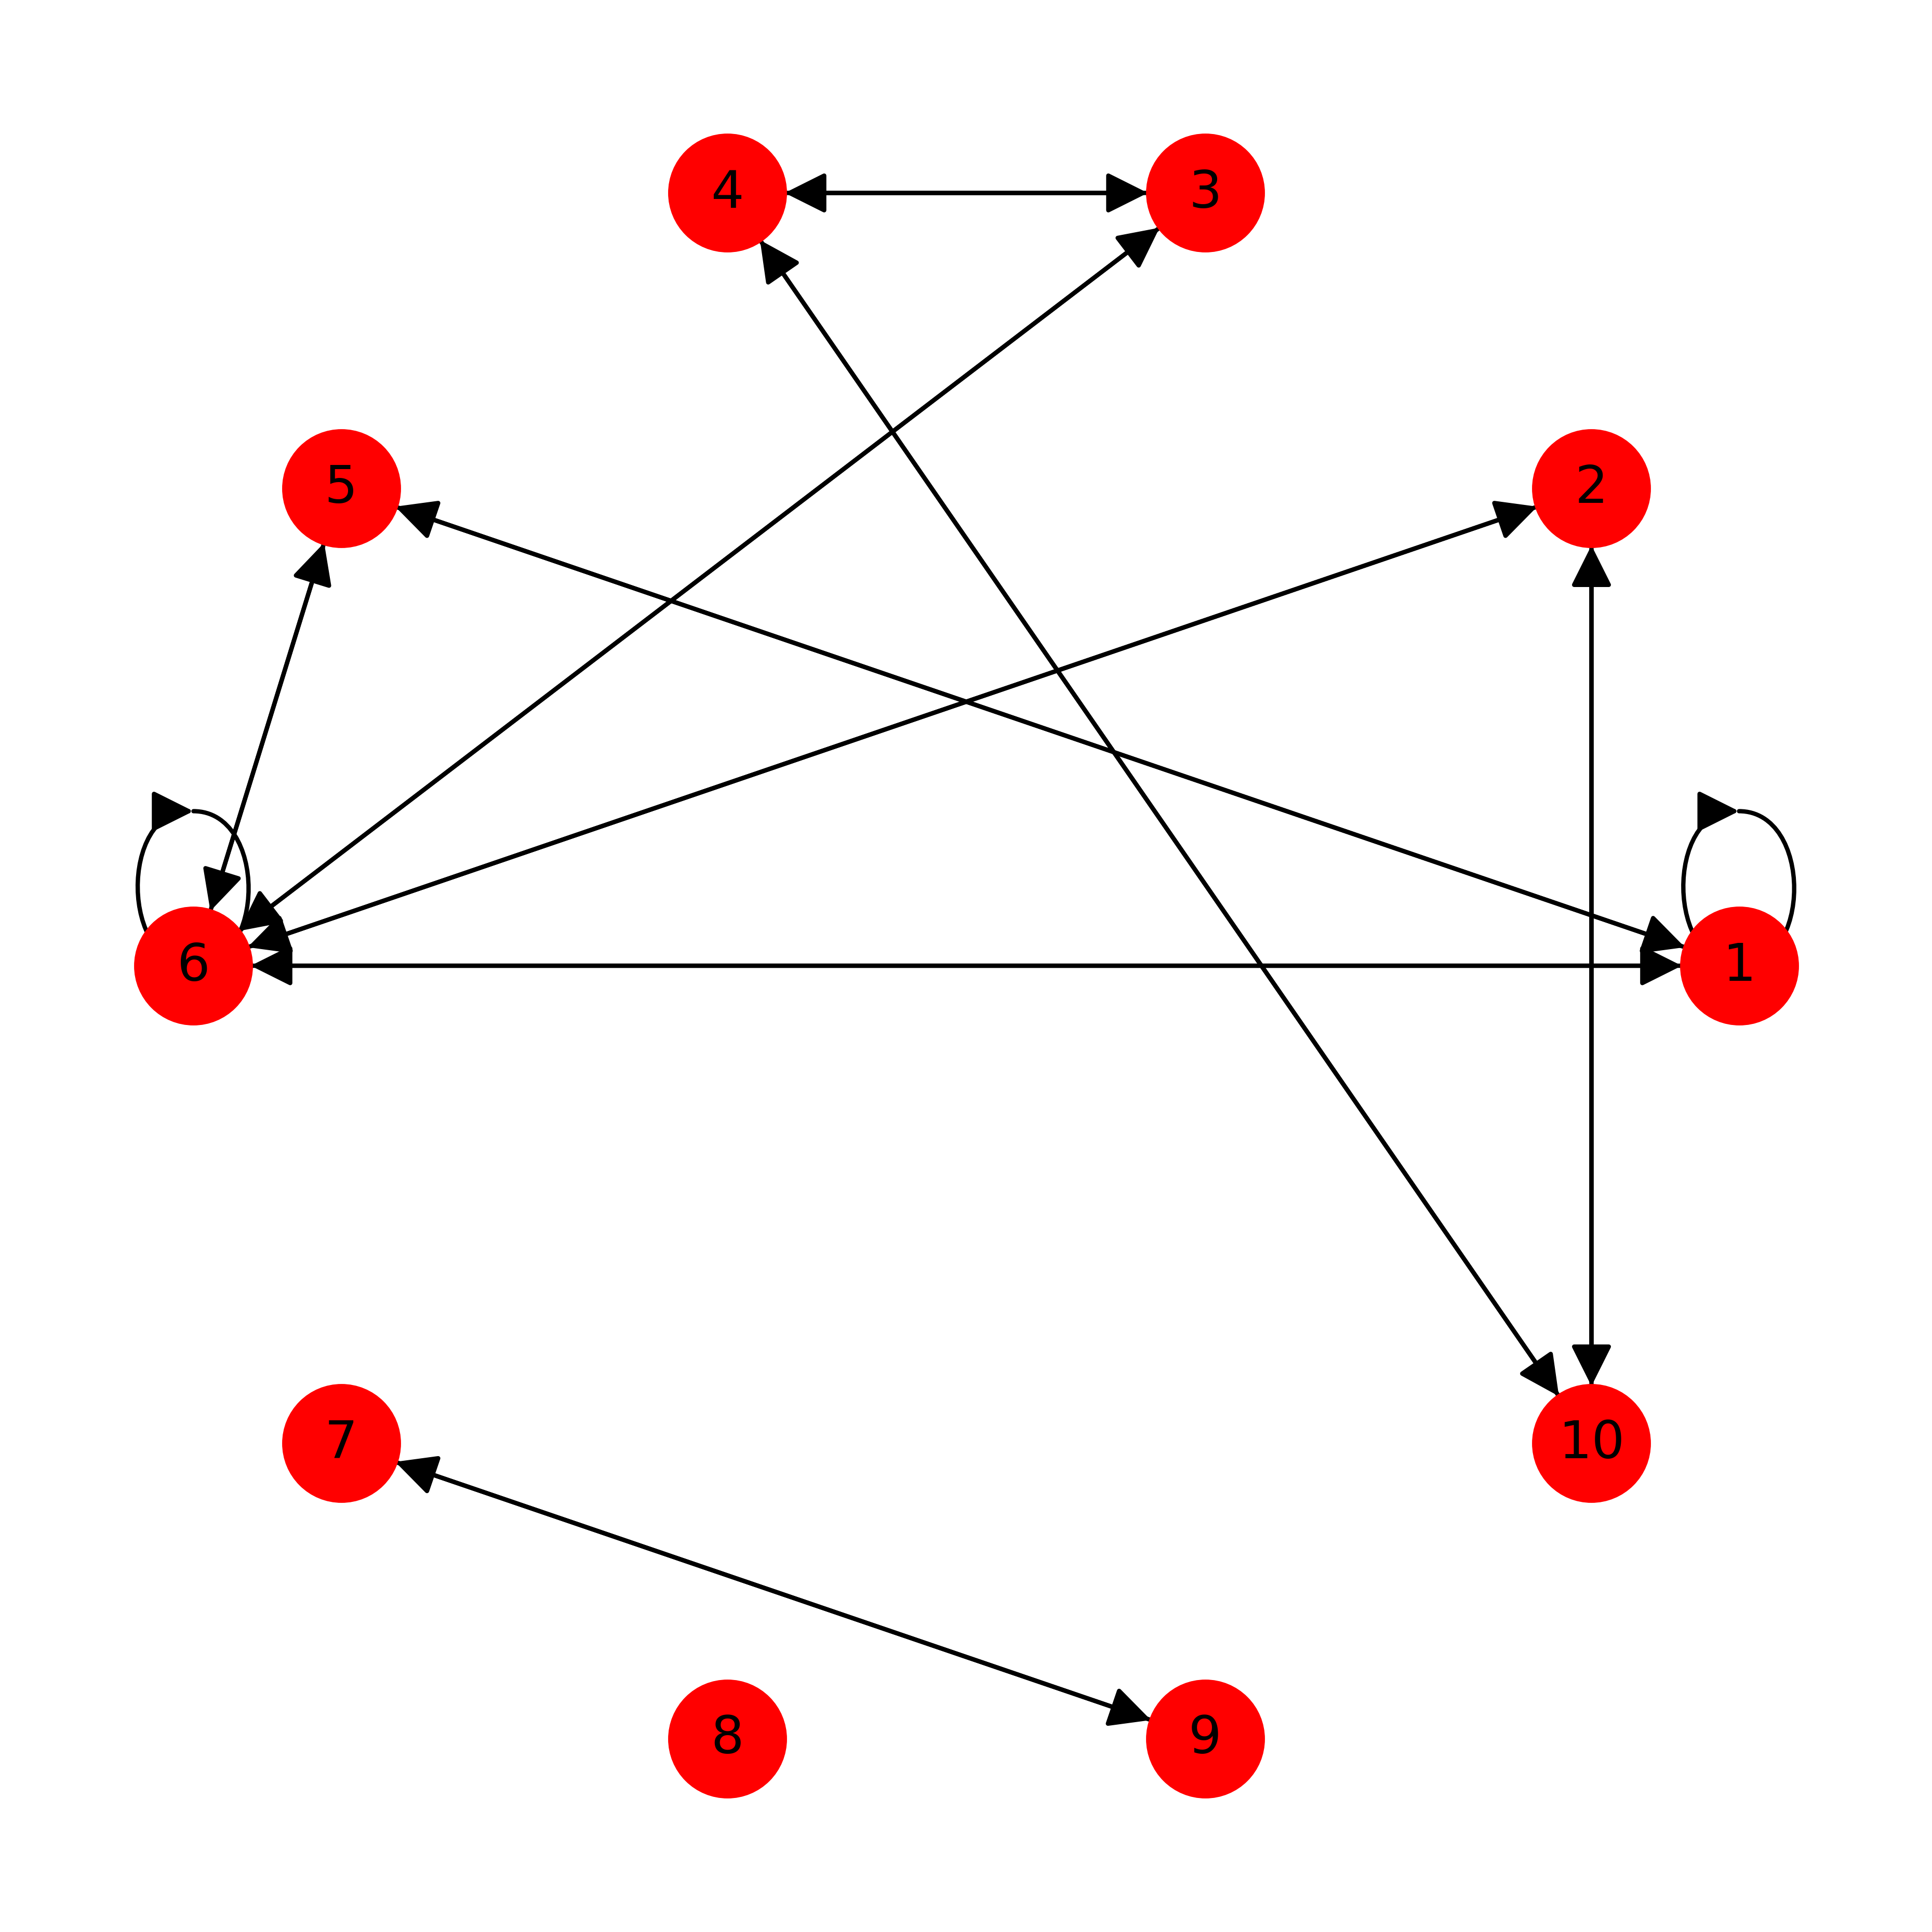
\includegraphics[width=0.4\linewidth]{img/11.png}
    \caption{Нерефлексивный, Нетранзитивный, Симметричный}
\end{figure}

\begin{figure}[h]
    \centering
    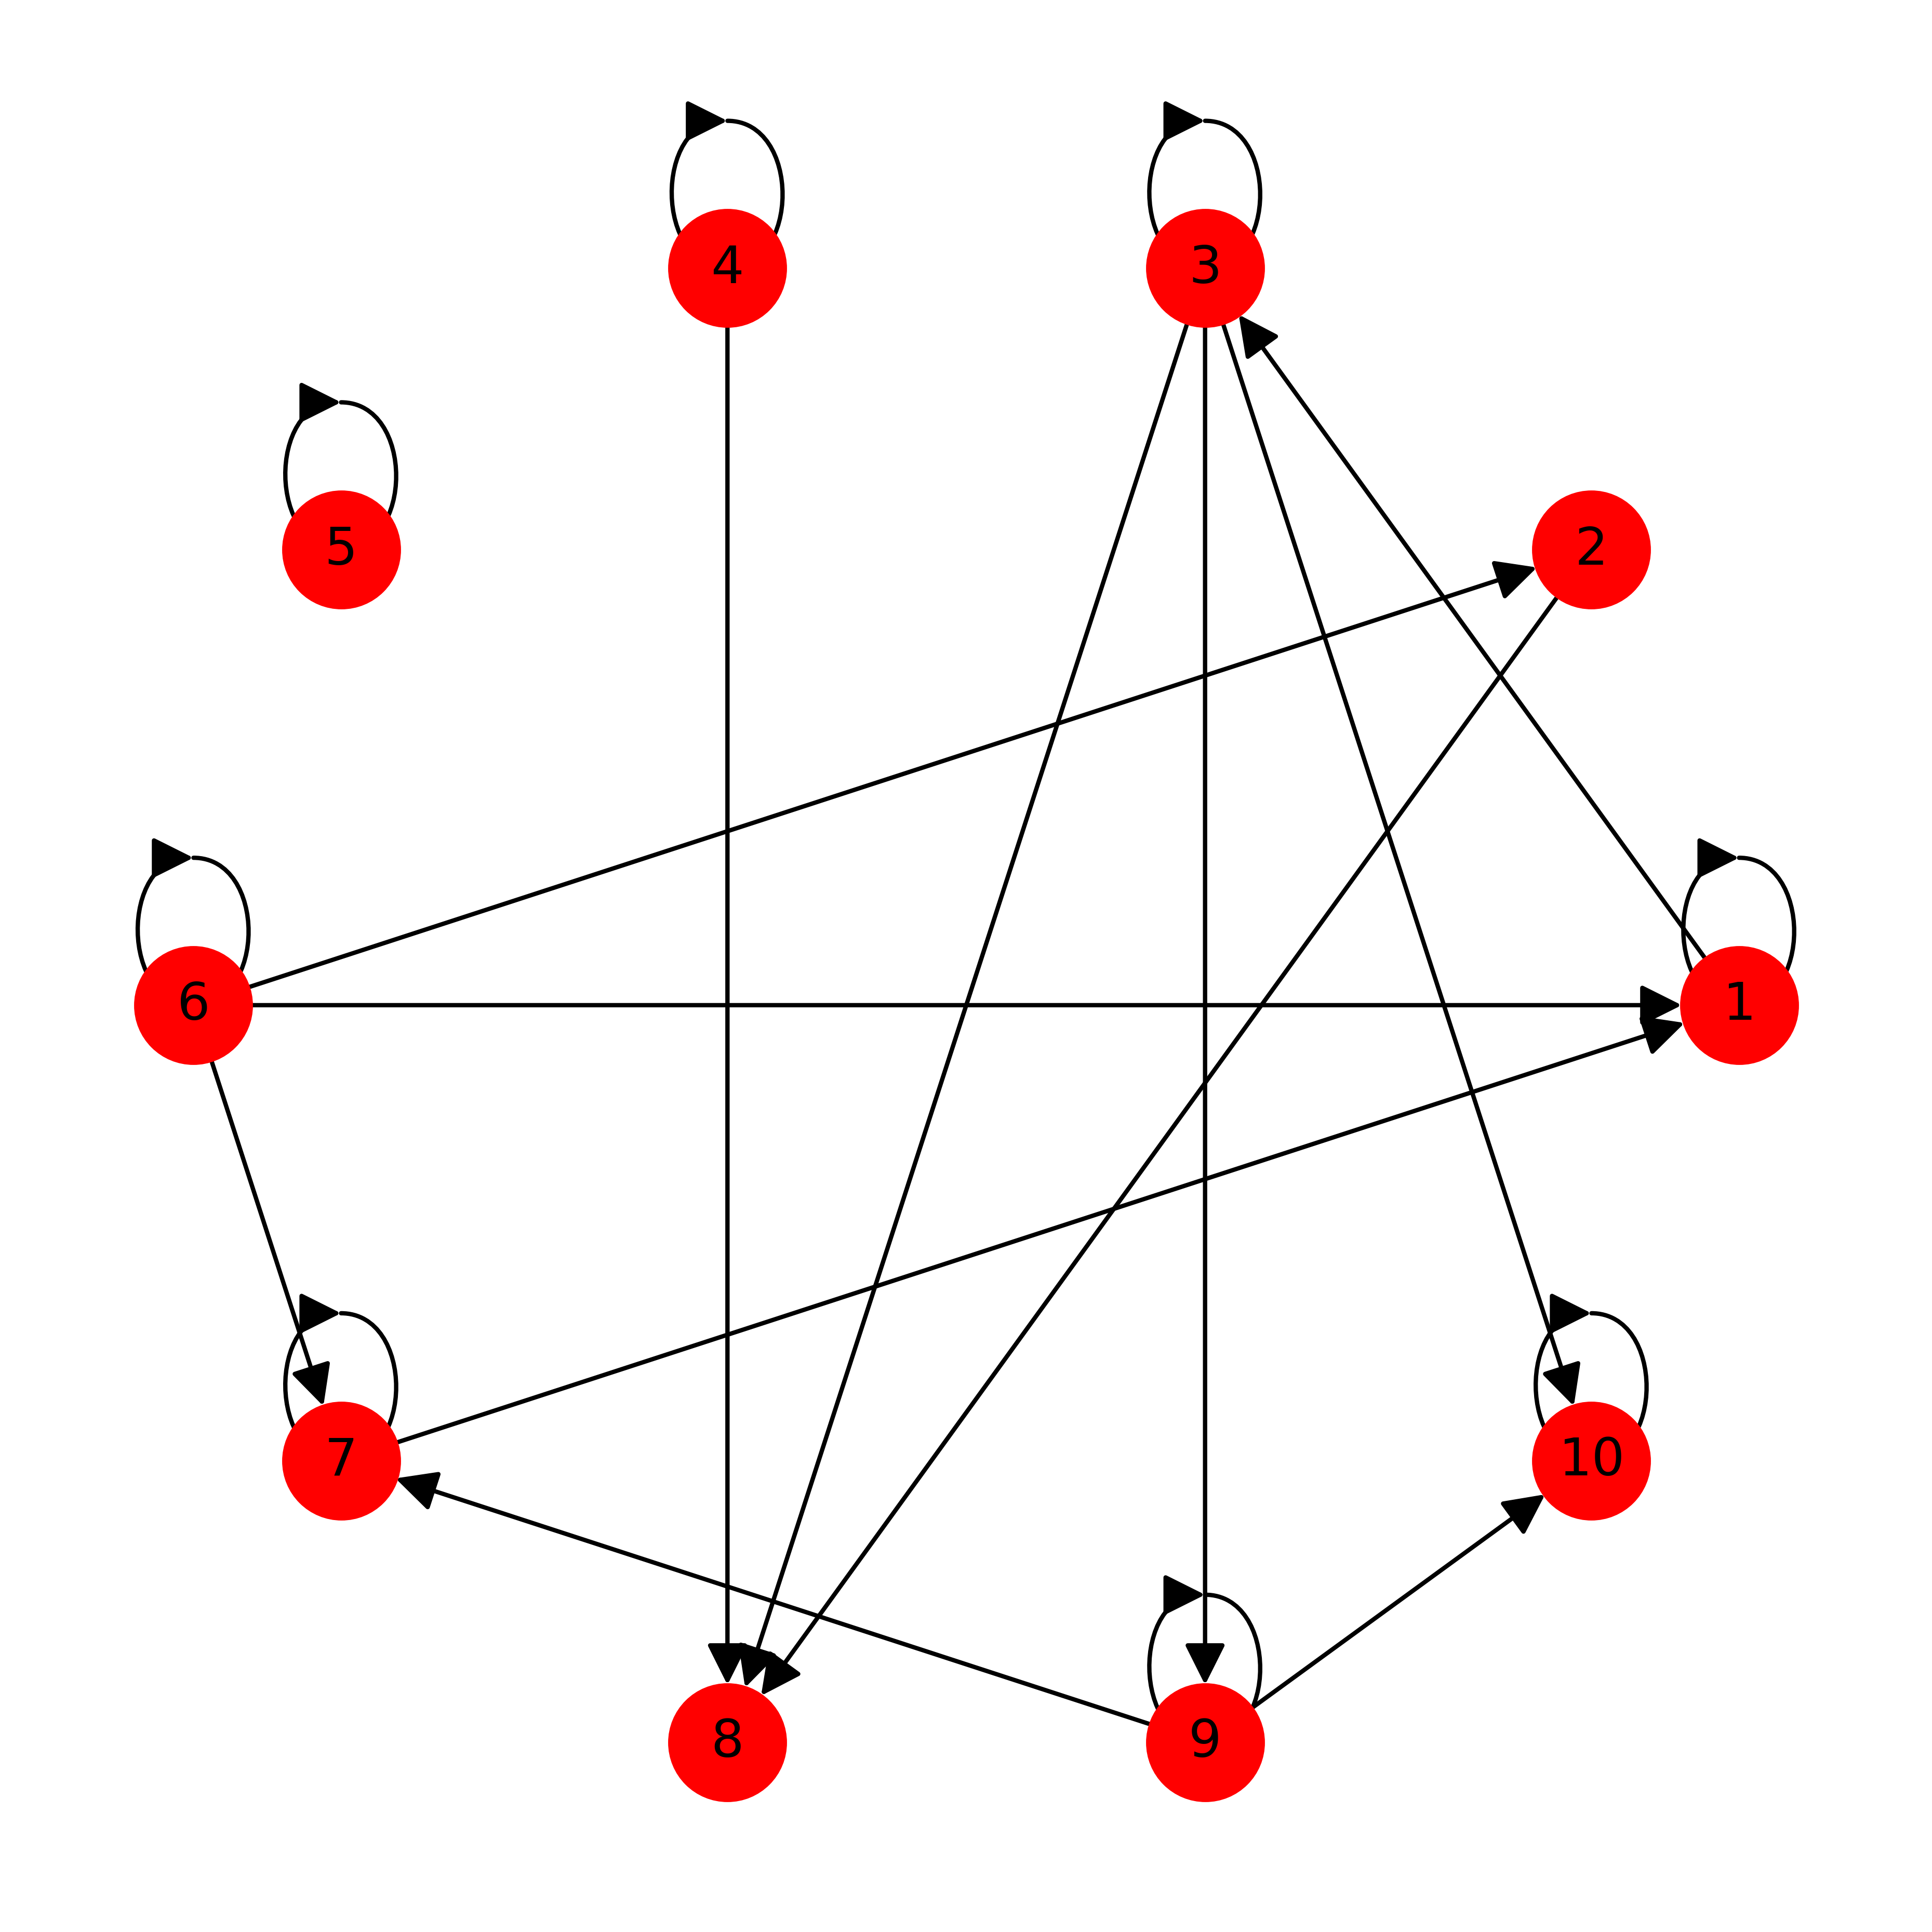
\includegraphics[width=0.4\linewidth]{img/12.png}
    \caption{Нерефлексивный, Нетранзитивный, Несимметричный, Антисимметричный}
\end{figure}

\begin{figure}[h]
    \centering
    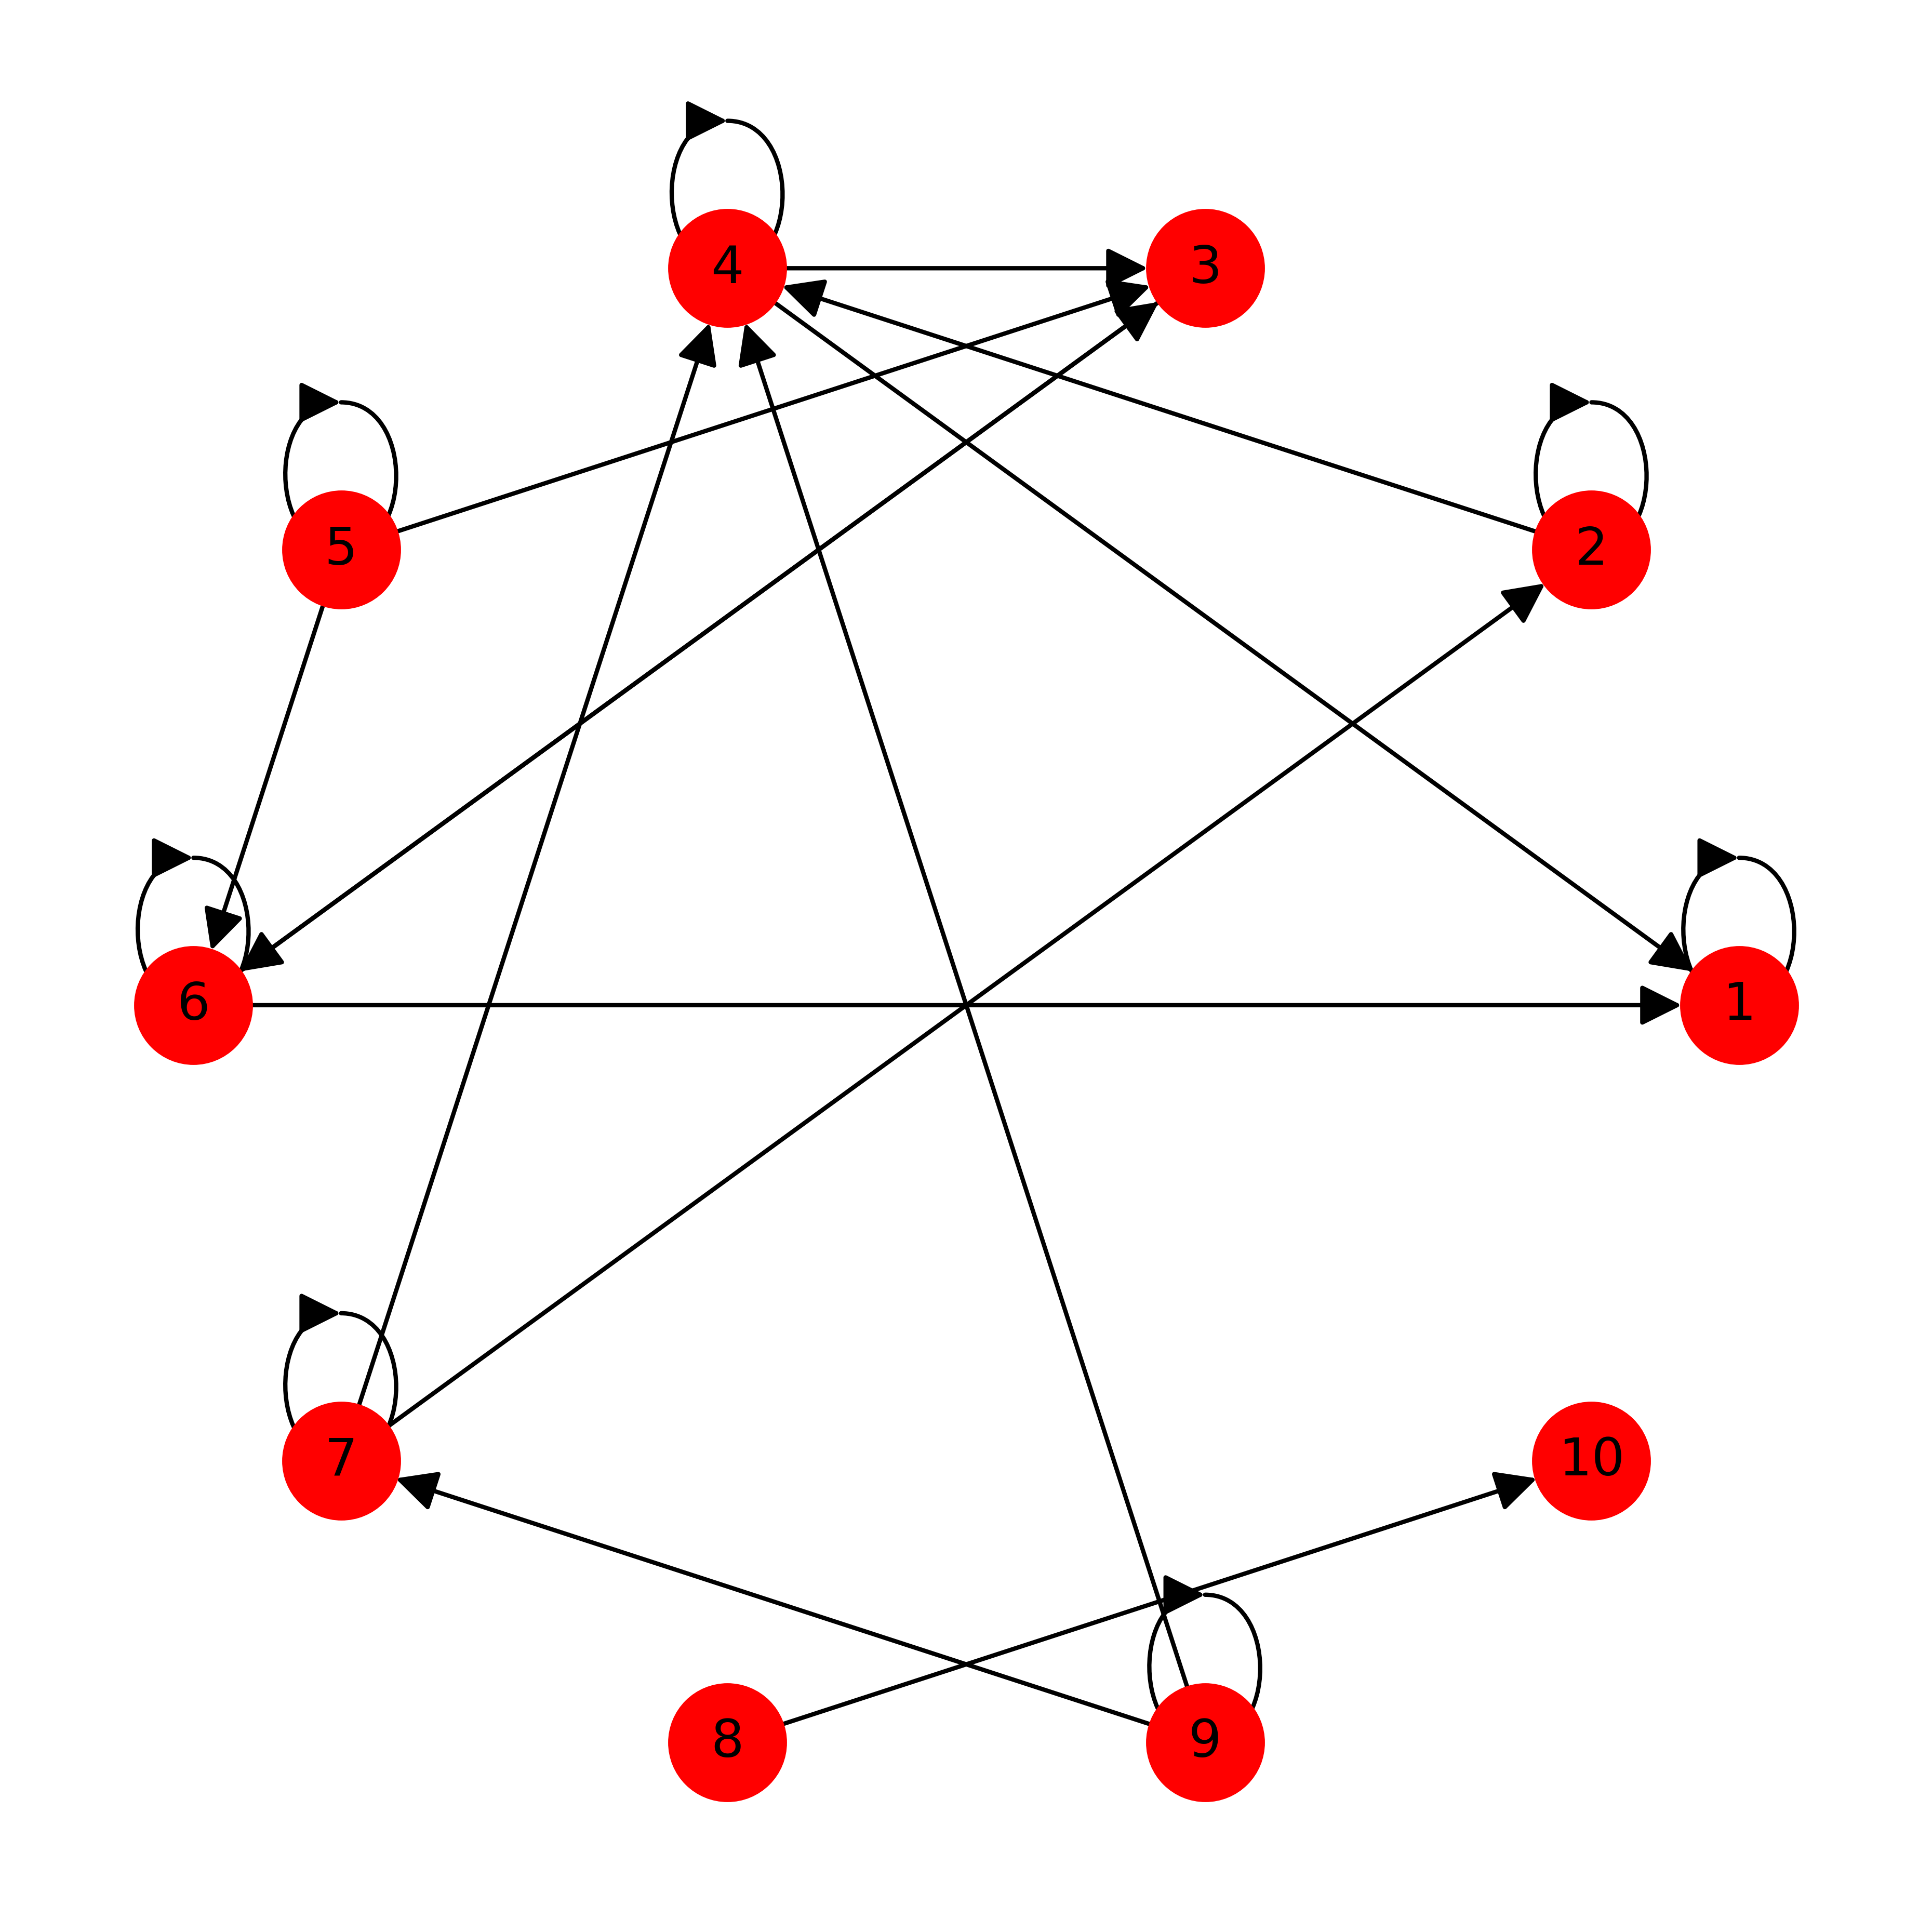
\includegraphics[width=0.4\linewidth]{img/13.png}
    \caption{Нерефлексивный, Нетранзитивный, Несимметричный}
\end{figure}

\begin{figure}[h]
    \centering
    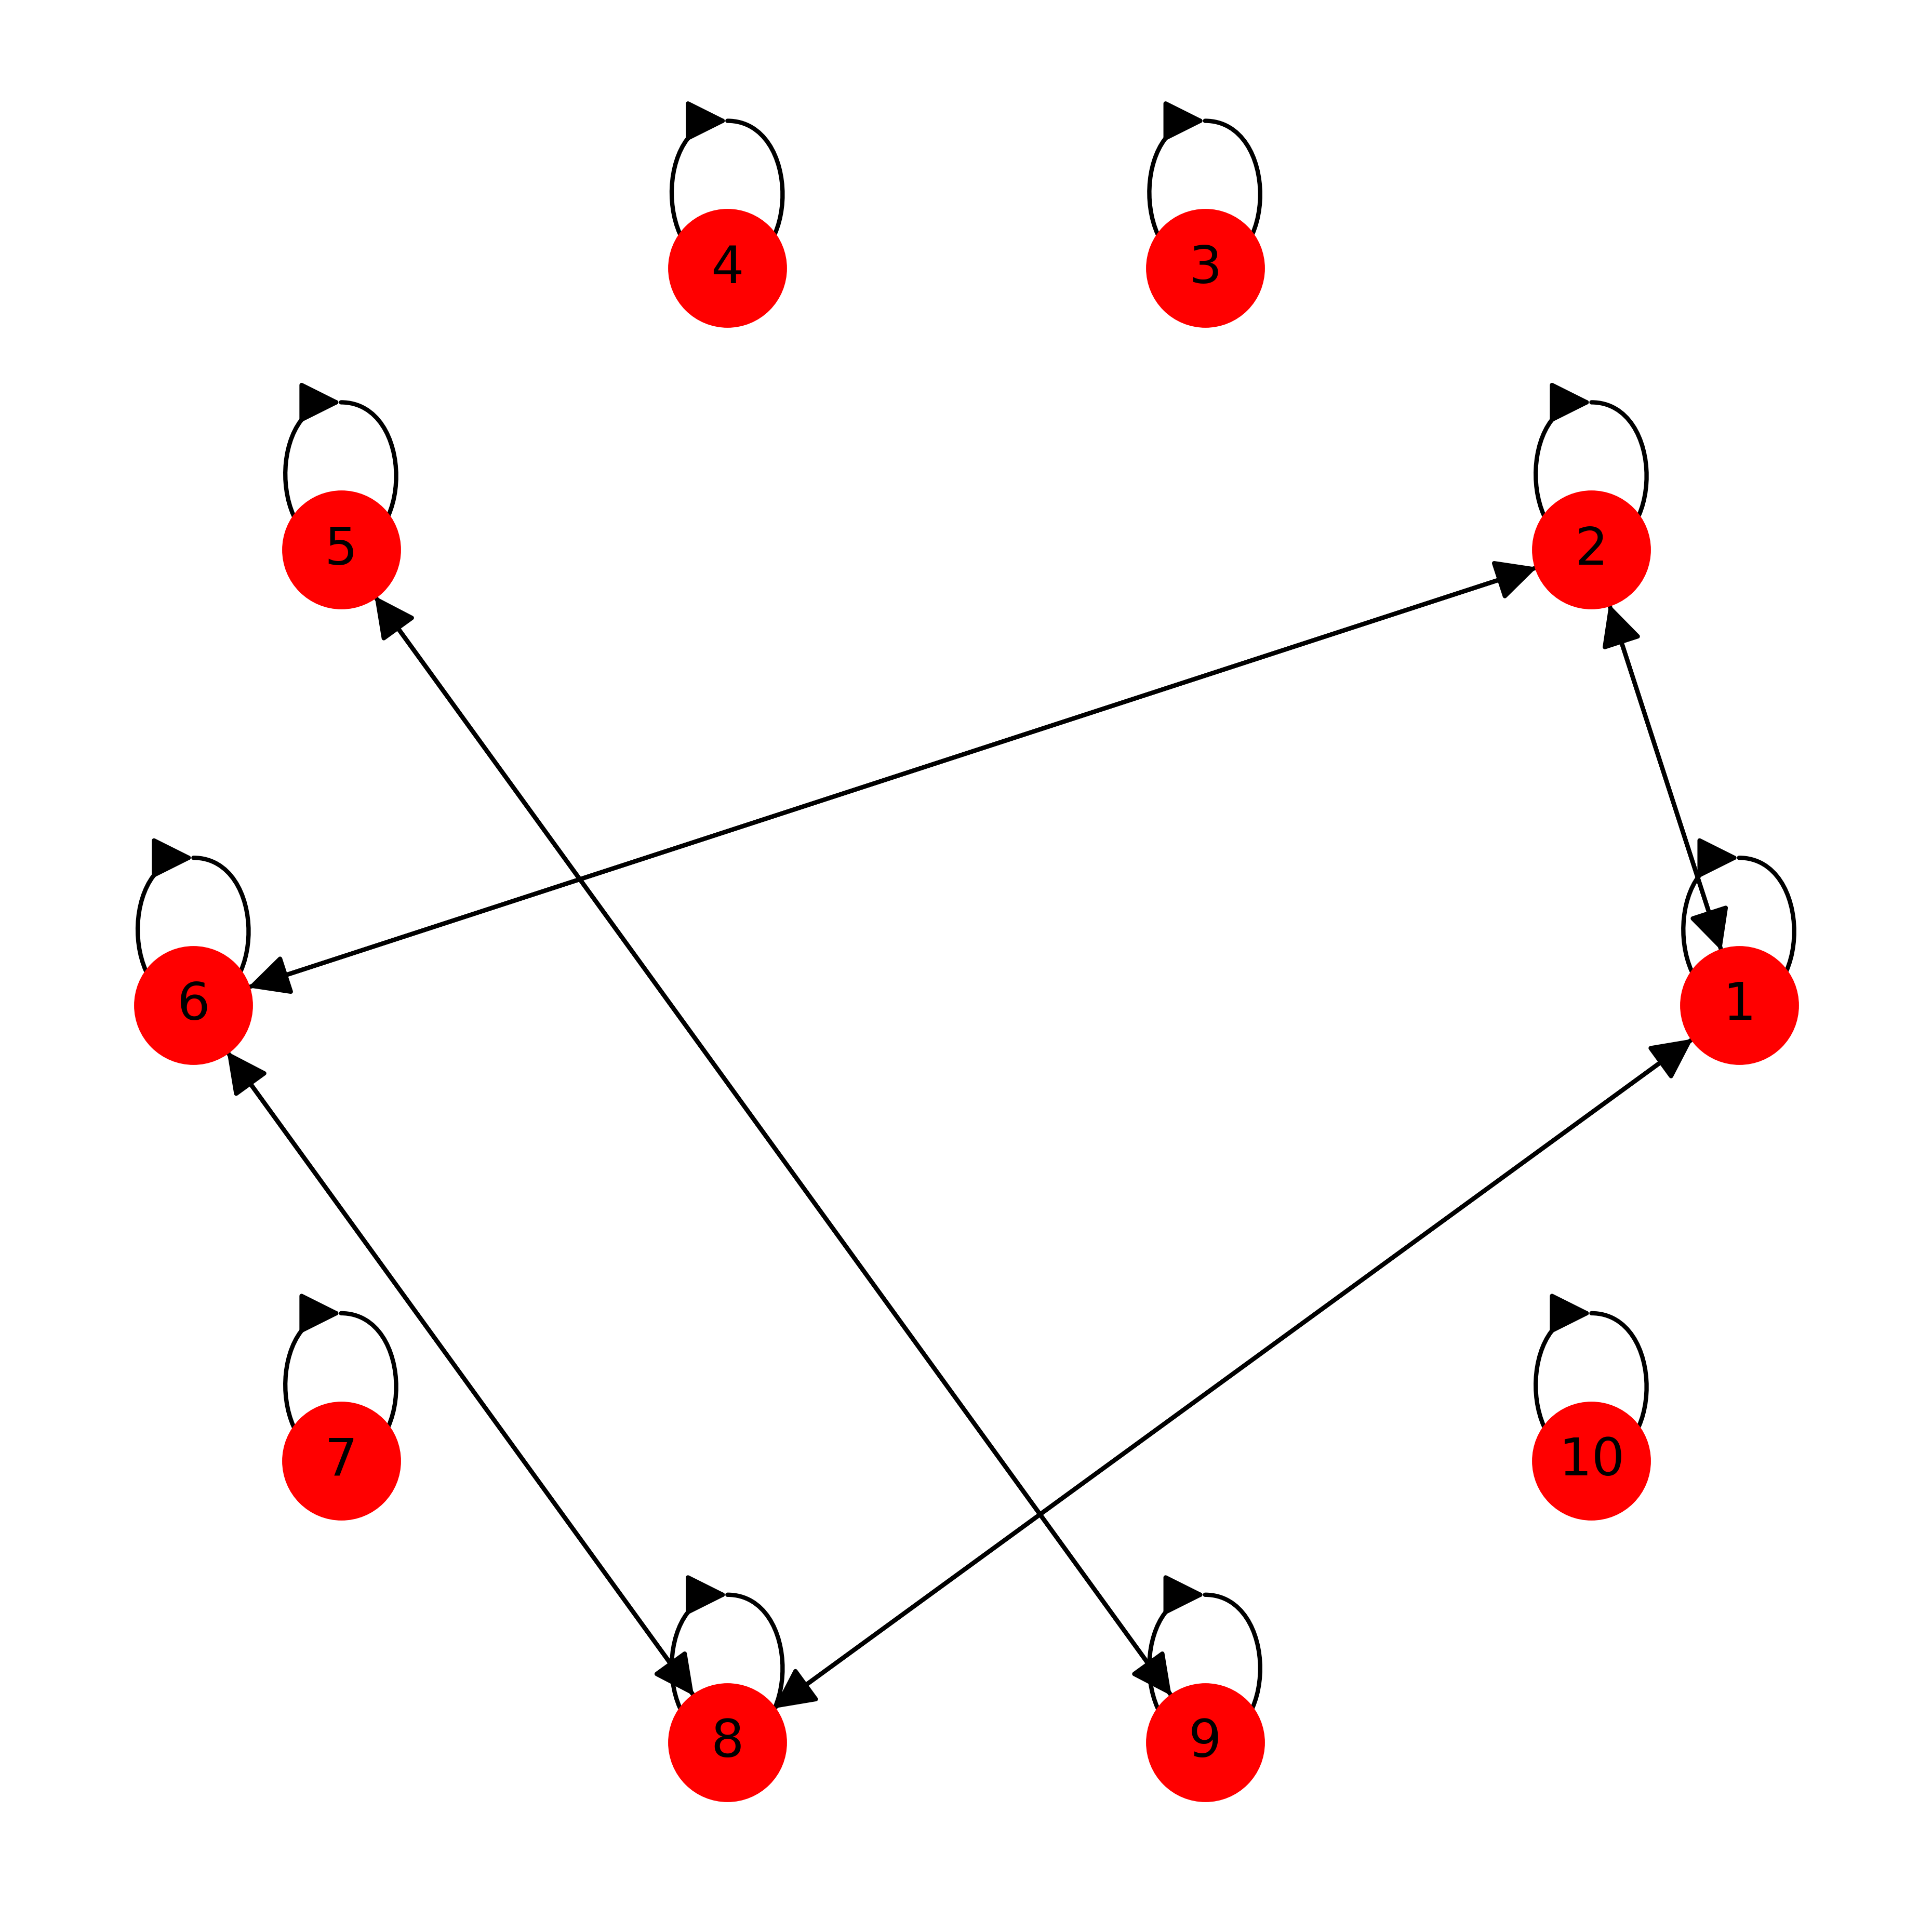
\includegraphics[width=0.4\linewidth]{img/14.png}
    \caption{Рефлексивный, Нетранзитивный, Симметричный}
\end{figure}

\begin{figure}[h]
    \centering
    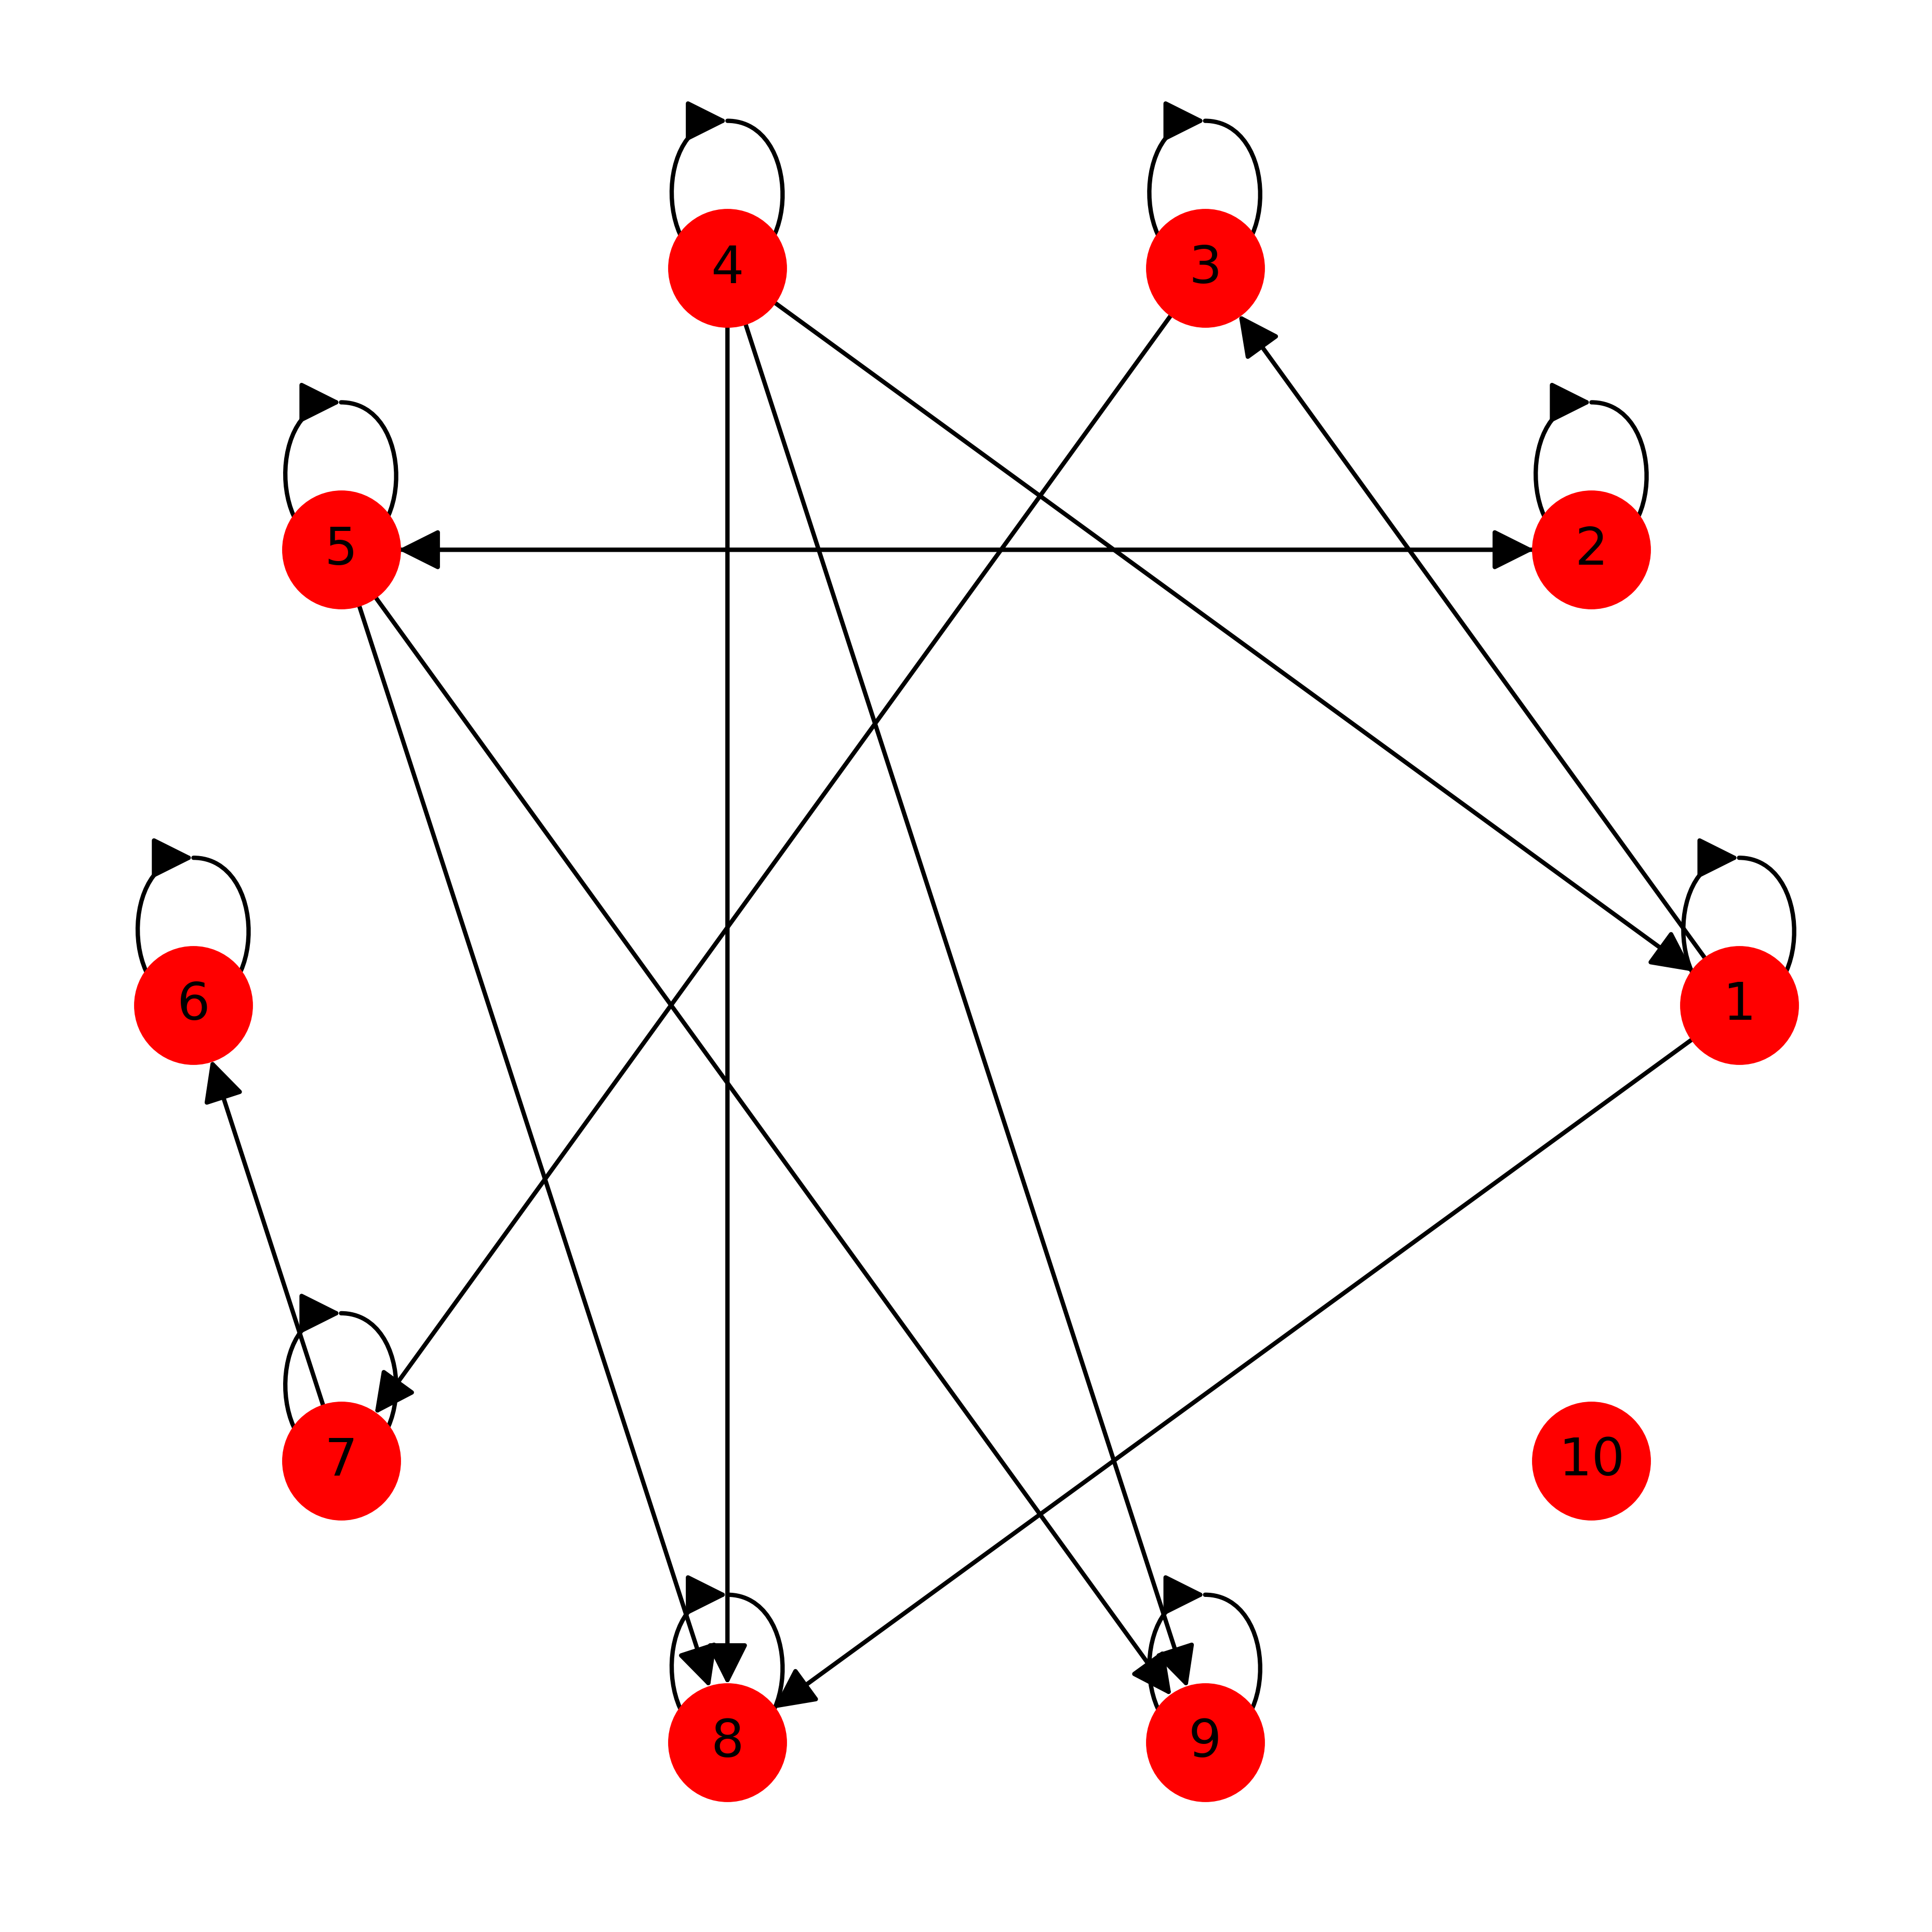
\includegraphics[width=0.4\linewidth]{img/15.png}
    \caption{Нерефлексивный, Нетранзитивный, Несимметричный}
\end{figure}


\end{document}